\documentclass[preprint2]{aastex62}
\graphicspath{ {./figs/} }
\usepackage{xspace, url}
%% \documentclass[twocolumn,linenumbers,trackchanges]{aastex61}
%%
\renewcommand{\figureautorefname}{Fig.}
\renewcommand{\sectionautorefname}{\S}
\renewcommand{\subsectionautorefname}{\S}
\renewcommand{\subsubsectionautorefname}{\S}
\renewcommand{\equationautorefname}{Eq.}
\renewcommand{\tableautorefname}{Table}
%% 
\newcommand{\Fig}[1]{\autoref{fig:#1}}
\newcommand{\Sec}[1]{\autoref{sec:#1}}
\newcommand{\Tab}[1]{\autoref{tab:#1}}
\newcommand{\Eq}[1]{\autoref{eq:#1}}
%% 
\newcommand{\z}[1]{$z \sim {#1}$}
\newcommand\vs{\ensuremath{\mathrm{vs.}}\xspace}
\newcommand{\FSPS}{{\sc FSPS}\xspace}
\newcommand{\pFSPS}{{\tt \textbf{python-fsps}}\xspace}
\newcommand{\CloudyFSPS}{{\tt \textbf{CloudyFSPS}}\xspace}
\newcommand{\Mappings}{{\sc Mappings-III}\xspace}
\newcommand{\Pegase}{\textsc{P{\'e}gase}\xspace}
\newcommand{\SB}{\textsc{Starburst-99}\xspace}
\newcommand{\Cloudy}{\textsc{Cloudy}\xspace}
\newcommand{\hii}{H\,{\sc ii}\xspace}
\newcommand{\nii}{[N\,{\sc ii}]\xspace}
\newcommand{\sii}{[S\,{\sc ii}]\xspace}
\newcommand{\oiii}{[O\,{\sc iii}]\xspace}
\newcommand{\oii}{[O\,{\sc ii}]\xspace}
\newcommand{\oi}{[O\,{\sc i}]\xspace}
\newcommand{\neiii}{[Ne\,{\sc iii}]\xspace}
\newcommand{\heii}{[He\,{\sc ii}]\xspace}
\newcommand{\hei}{[He\,{\sc i}]\xspace}
\newcommand{\civ}{C\,{\sc iv}\xspace}
\newcommand{\siIII}{Si\,{\sc iii}\xspace}
\newcommand{\siII}{Si\,{\sc ii}\xspace}
\newcommand{\suIII}{Si\,{\sc ii}\xspace}
\newcommand{\ciii}{C\,{\sc iii}\xspace}
\newcommand{\cii}{C\,{\sc ii}\xspace}
\newcommand\Lsun{\ensuremath{\,\mathrm{L_{\sun}}}\xspace}
\newcommand\Msun{\ensuremath{\,\mathrm{M_{\sun}}}\xspace}
\newcommand{\ha}{\ensuremath{\mathrm{H\alpha}}\xspace}
\newcommand{\hb}{\ensuremath{\mathrm{H\beta}}\xspace}
\newcommand{\logten}{\ensuremath{\log_{10}}}
\newcommand{\logz}{\ensuremath{\logten \mathrm{Z}/\mathrm{Z}_{\sun}}\xspace}
\newcommand{\logZeq}[1]{\ensuremath{\logten \mathrm{Z}/\mathrm{Z}_{\sun} = #1}}
\newcommand{\ang}{\ensuremath{\mbox{\AA}}\xspace}
\newcommand{\logQ}[1]{\ensuremath{\logten Q_{#1}}}
\newcommand{\QH}{\ensuremath{Q_{\mathrm{H}}}\xspace}
\newcommand{\QHe}{\ensuremath{Q_{\mathrm{He}}}\xspace}
\newcommand{\QHat}{\ensuremath{\hat{Q}_{\mathrm{H}}}\xspace}
\newcommand{\QHehat}{\ensuremath{\hat{Q}_{\mathrm{He}}}\xspace}
\newcommand{\U}{\ensuremath{\mathcal{U}_{0}}\xspace}
\newcommand{\logU}{\ensuremath{\logten \mathcal{U}_0}}
\newcommand{\logUeq}[1]{\ensuremath{\logten \mathcal{U}_0 = #1}}
\newcommand{\kms}{\ensuremath{\;\mathrm{km}\;\mathrm{s}^{-1}}\xspace}
\newcommand{\Myr}{$\,$Myr\xspace}
\newcommand{\Gyr}{$\,$Gyr\xspace}
%%
\newcommand{\vdag}{(v)^\dagger}
\newcommand\aastex{AAS\TeX}
\newcommand\latex{La\TeX}
%%%%%%%%%%%%%%%%%%%%%%%%%%%%%%%%%%%%%%%%%%%%%%%%%%%%%%%%%%%%%%%%%%%%%%%%%%%%%%%%
%%
%\received{July 1, 2016}
\revised{\today}
%\accepted{\today}
%\submitjournal{ApJ}
%%
\shorttitle{LIER-like emission lines from post-AGB stars}
\shortauthors{Byler et al.}
%%
%%%%%%%%%%%%%%%%%%%%%%%%%%%%%%%%%%%%%%%%%%%%%%%%%%%%%%%%%%%%%%%%%%%%%%%%%%%%%%%%
\begin{document}
\title{Self-consistent predictions for LIER-like emission lines from post-AGB stars}
%%%%%%%%%%%%%%%%%%%%%%%%%%%%%%%%%%%%%%%%%%%%%%%%%%%%%%%%%%%%%%%%%%%%%%%%%%%%%%%%
%%
\author[0000-0002-7392-3637]{Nell Byler}
\affil{Department of Astronomy, University of Washington, Box 351580, Seattle, WA 98195, USA}
%% 
\author[0000-0002-1264-2006]{Julianne J. Dalcanton}
\affil{Department of Astronomy, University of Washington, Box 351580, Seattle, WA 98195, USA}
%%
\author[0000-0002-1590-8551]{Charlie Conroy}
\affil{Department of Astronomy, Harvard University, Cambridge, MA, USA}
%%
\author{Benjamin D. Johnson}
\affil{Department of Astronomy, Harvard University, Cambridge, MA, USA}
%%
\author{Jieun Choi}
\affil{Department of Astronomy, Harvard University, Cambridge, MA, USA}
%%
\author{Aaron Dotter}
\affil{Department of Astronomy, Harvard University, Cambridge, MA, USA}
%%
\author[0000-0001-9306-6049]{Philip Rosenfield}
\affil{Department of Astronomy, Harvard University, Cambridge, MA, USA}
%%
%%%%%%%%%%%%%%%%%%%%%%%%%%%%%%%%%%%%%%%%%%%%%%%%%%%%%%%%%%%%%%%%%%%%%%%%%%%%%%%%
\begin{abstract}

In early type galaxies (ETGs), emission from warm ionized gas, characterized by Low Ionization Emission Regions (LIERs), was originally attributed to a central, low-luminosity active galactic nuclei (AGN). However, the recent discovery of spatially-extended LIER emission suggests ionization by both a central source and something with a stellar-like radial distribution. For passively-evolving galaxies with old stellar populations, hot post-Asymptotic Giant Branch (AGB) stars are the only viable source of ionizing photons. In this work, we present the first prediction of LIER-like emission from post-AGB stars that is based on fully self-consistent stellar evolution models and photoionization modelling. We show that models where post-AGB stars are the dominant source of ionizing photons are able to reproduce the nebular emission signatures observed in ETGs. Our models produce LIER-like emission line ratios in standard optical diagnostic diagrams and produce \ha equivalent widths (EWs) of order 0.1-10\ang, in agreement with observations. Models with with delayed-$\tau$ star formation histories with $\tau$ between 0 and 0.5\Gyr, ages between 2 and 13\Gyr and metallicities between \logZeq{-1} and 0.25 are able to reproduce LIER-like emission line ratios and EWs without any tuning. These same models accurately reproduce the optical colors and absorption indices typical of the ETG population.%, and we discuss the implication for the stellar populations responsible for the UV-excess observed in some ETGs. Finally, we test the sensitivity of the post-AGB phase and the resultant LIER-like emission to the mass loss efficiency, convective mixing efficiency, and rotation rate used in the MIST isochrones. We find that increasing the mass loss efficiency factor can increase observed \ha EWs from post-AGB stars. 

\end{abstract}
\keywords{Galaxies --- galaxies: emission lines --- galaxies: abundances --- galaxies: ISM}
%%%%%%%%%%%%%%%%%%%%%%%%%%%%%%%%%%%%%%%%%%%%%%%%%%%%%%%%%%%%%%%%%%%%%%%%%%%%%%%%
\section{Introduction} \label{sec:intro}

Early type galaxies (ETGs) are usually assumed to be gas-poor, passively-evolving systems. However, we now know that ETGs can harbor reservoirs of diffuse ionized gas \citep{Sarzi+2006, Singh+2013, Kehrig+2012, Papaderos+2013}. The source of ionization in these systems has been under recent debate, with explanations that include the heat transfer from hot to cold gas \citep{Heckman+1981}, shock waves \citep{Koski+1976, Dopita+1995, Allen+2008}, central active galactic nuclei \citep[AGN; ][]{Ferland+1983, Halpern+1983, Heckman+1998, Ho+1999, Kauffmann+2003b, Kewley+2006, Ho+2009}, or evolved stellar sources \citep{Binette+1994, Taniguchi+2000}. However, current research supports the view that for most galaxies, the gas excitation is driven by photoionization from evolved stars and fast shocks on extended kpc scales, with additional contributions from low-luminosity AGN on nuclear scales \citep[e.g., ][]{Pandya+2017}.

The low-ionization emission was originally discovered in the nuclear regions of galaxies, and then attributed to AGN-related activity. However, recent spatially resolved spectroscopy has revealed that low-ionization emission regions (LIERs) are not always centrally concentrated and instead can be spatially extended over ${\sim}\mathrm{kpc}$ scales \citep{Belfiore+2016, James+2015, Gomes+2016}. While central LIER emission is likely still attributable to low-luminosity AGN activity \citep{Sarzi+2010, Belfiore+2016, Kormendy+2013, Pandya+2017}, it has been suggested that hot evolving stars, which are the primary source of ionizing photons when main sequence stars are absent, are responsible for the spatially-extended LIER emission \citep{Binette+1994, Stasinska+2008,Sarzi+2010, Yan+2012, Woods+2014, Johansson+2016}.

In the quiescent stellar populations that dominate ETGs and spiral bulges, the source of ionizing photons cannot be young massive stars. Instead, the ionization is likely due to evolving low- and intermediate-mass stars. There are two main candidates for stars that are hot enough and either luminous or numerous enough to power significant ionization. The first is extreme horizontal branch (EHB) stars, a sub-group of HB stars, the evolutionary stage immediately following the Red Giant Branch (RGB) phase. Stars with initial masses between 0.8 and 2\Msun undergo a helium flash and begin core-helium fusion on the HB. Stars that have experienced more mass loss during their RGB evolution begin their HB phase with less massive hydrogen shells, producing hot or ``extreme'' HB stars. These stars are relatively faint when compared to other possible ionizing sources (50-100\Lsun) but are very numerous and relatively long-lived, with lifetimes $\sim 10^8$ years. 

The second stellar candidate is post-Asymptotic Giant Branch (AGB) stars, which are stars with initial masses between 0.8 and 8\Msun that have left the AGB and are evolving horizontally across the HR diagram towards very hot temperatures ($\sim10^5$ K) before cooling down to form white dwarfs. Although they are not as long-lived as EHB stars ($\sim10^3-10^7$ years), post-AGB stars are much more luminous ($\mathrm{L}_{bol} = 10^{2-4}\Lsun$) and possibly hotter (see reviews in \citealp{OConnell+1999, Grevesse+2010}; also \citealp{Bressan+2012}). 

As an ionizing source, the term ``post-AGB'' sometimes encompasses a broader category of hot evolving stars that includes early-AGB stars, AGB-Manque stars, pre-planetary nebulae and white dwarfs \citep{Stasinska+2008}. Broader terms for this larger category include ``hot old low mass evolved stars'' \citep[HOLMES; ][]{Fernandes+2011} and ``hot post-horizontal branch stars,'' \citep[HPHB; ][]{Rosenfield+2012}.

%These different subclasses include stars with a range of temperatures, luminosities, and lifetimes, not all of which are equally effective at driving ionization. They can however, produce significant UV flux longwards of 912\ang, even for old stellar populations. This flux has been detected with facilities like GALEX, SWIFT, or IUE at low redshift, or with optical or NIR facilities for highly redshifted galaxies. In some cases the UV flux is seen to rise towards short wavelengths, in a phenomenon referred to as the ``UV upturn''.
%
%The source of the UV-upturn phenomenon in ETGs is still debated, with suggestions that include a population of helium-rich stars or stars who have had their atmospheres stripped away through binary interactions. The manifestation of the UV upturn phenomenon is highly variable, occuring in roughly 3-10\% of local ETGs (depending on selection criteria, see for example \citealp{Smith+2014}), independent of whether the ETG hosts LIER-like emission. Likewise, recent work has found that ETGs with similar morphologies and optical colors can display a wide range of NUV-optical colors \citep{Yi+2005, Kaviraj+2007, Schawinski+2007}. 
%
%All of these UV-emission phenomena in old stellar populations (photoionization to produce LIER-like emission, UV upturn, diverse UV-optical colors) are likely to be driven by stars of similar masses (${\sim}$3, 2, and 1 \Msun for 2, 6, and 12\Gyr old populations) given the rapidity of post-RGB evolution. As such, a self-consistent model of the stellar and nebular spectral energy distribution (SED) should be able to simultaneously reproduce the UV and optical colors and emission line ratios of LIER-like galaxies, if HPHB models are correct.
%
%Calculating the needed self-consistent models of UV emission requires making predictions for the nebular emission produced by ionization from the hottest HPHB phases.
%
Estimates of LIER-like emission based on the numbers of ionizing photons produced by post-AGB stars in stellar evolution models indicate \ha equivalent widths of order a few angstroms for ETGs \citep{Maraston+2005, CidFernandes+2011, Belfiore+2016,Gomes+2016}. However, these current estimates are first-order calculations assuming case-B recombination for fixed-temperature gas. In \citet{Byler+2017}, we showed that accounting for temperature variations is essential when predicting emission line strengths. Accurate predictions of emission line luminosities and equivalent widths require the consideration of metallicity- and age-driven changes to the ionizing spectrum and metallicity-driven changes in the gas phase abundances. 

There have been a few attempts to use photoionization modelling to explore the origin of LIER-like emission. In \citet{Byler+2017}, we demonstrated that our nebular model was able to reproduce LIER-like emission line ratios using older populations where hot evolved stars are the dominant ionization source. This work confirmed that current stellar evolution models and stellar atmospheres are capable of producing appropriately hard ionizing spectra. Similarly, \citet{Hirschmann+2017} used old stellar populations to predict emission line ratios from evolved stars to explore the relative contribution from star formation, AGN, and post-AGB stars to the cosmic evolution of the BPT emission line ratios. While the work in \citet{Byler+2017} and \citet{Hirschmann+2017} provides useful insight into the physical origin of observed optical line ratios, they do not reveal anything about the nature of LIER-like emission or post-AGB stars as ionizing sources, nor do they show simultaneous consistency with the broader emission from the larger HPHB population.

In general, the models used for stars during the post-AGB phase are computed separately from the rest of the stars evolution. In the MESA Isochrones \& Stellar Tracks \citep[MIST; ][]{Dotter+2016, Choi+2016}, stellar evolution for low-mass stars is continuously computed from the pre-main sequence phase to the end of white dwarf (WD) cooling phase. The temperatures, luminosities, and lifetimes associated with the post-AGB phase are a natural prediction of the stellar models, and produce colors that are well-matched with observations throughout their evolution.

In this work, we present the first prediction of LIER-like emission from post-AGB stars that is based on fully self-consistent stellar and photoionization modelling. We build on the work from \citet{Byler+2017}, who paired the population synthesis models from the Flexible Stellar Population Synthesis code \citep[\FSPS; ][]{Conroy+2009} with photoionization models from \Cloudy \citep{Ferland+2013} to self-consistently model the flux from star-forming galaxies. As we show here, this model can simultaneously reproduce the nebular emission signatures of star forming galaxies and LIER-like emission signature observed in ETGs. We also show that this model accurately reproduces the optical properties observed in the ETG population.

We describe the stellar and nebular model in \S\ref{sec:model}. In \S\ref{sec:stars}, we introduce the ionizing radiation produced by hot evolved stars (\S\ref{sec:stars:ion}) and demonstrate that our models produce LIER-like equivalent widths and emission line ratios (\S\ref{sec:stars:emis}). In \S\ref{sec:stars:continuum} we show that our models also reproduce observed ETG optical colors and absorption line properties. Our conclusions are summarized in \S\ref{sec:conclusions}.

%%%%%%%%%%%%%%%%%%%%%%%%%%%%%%%%%%%%%%%%%%%%%%%%%%%%%%%%%%%%%%%%%%%%%%%%%%%%%%%%
\section{Description of Model}\label{sec:model}

We use the publicly available \CloudyFSPS\footnote{Read the documentation at \url{http://nell-byler.github.io/cloudyfsps/}} \citep{cloudyFSPSv1} from \citet{Byler+2017} to compute the line and continuum emission for stellar populations from \FSPS using the photoionization code \Cloudy. The nebular model is described in detail in \citet{Byler+2017}, but we briefly summarize the process of generating model spectra in this section. We describe the stellar models in \S\ref{sec:model:stellar} and the nebular model in \S\ref{sec:model:neb}.

%===============================================================================
\subsection{The stellar model}\label{sec:model:stellar}

We generate the underlying stellar spectra using the Flexible Stellar Population Synthesis package\footnote{\url{https://github.com/cconroy20/fsps}} \citep[FSPS; ][]{Conroy+2009, Conroy+2010} via the Python interface, \pFSPS \citep{pythonFSPSdfm}. We adopt a Kroupa initial mass function \citep[IMF;][]{Kroupa+2001} with an upper and lower mass limit of 120\Msun and 0.08\Msun, respectively. We use the default parameters in \FSPS\footnote{\FSPS GitHub commit hash \texttt{3656df5}; \pFSPS GitHub commit hash \texttt{57e59f7}} unless otherwise noted.

We use evolutionary tracks from the MESA Isochrones \& Stellar Tracks \citep[MIST\footnote{Documentation, packaged model grids, and a web interpolator are available at \url{http://waps.cfa.harvard.edu/MIST/}};][]{Dotter+2016, Choi+2016}, single-star stellar evolutionary models which include the effect of stellar rotation. The evolutionary tracks are computed using the publicly available stellar evolution package Modules for Experiments in Stellar Astrophysics \citep[MESA v7503;][]{Paxton+2011,Paxton+2013, Paxton+2015} and the isochrones are generated using Aaron Dotter's publicly available \texttt{iso} package on github\footnote{available at \url{https://github.com/dotbot2000/iso}}. The MIST models cover ages from $10^5$ to $10^{10.3}$ years, initial masses from $0.1$ to $300\,$\Msun, and metallicities in the range of $-2.0 \leq$ $[\mathrm{Z}/\mathrm{H}]$ $\leq 0.5$. Abundances are solar-scaled, assuming the \citet{Asplund+2009} protosolar birth cloud bulk metallicity, for a reference solar value of $\mathrm{Z}_{\odot} = 0.0142$.  A complete description of the models can be found in \citet{Choi+2016}.

Stellar evolution is continuously computed from the pre-main sequence phase to the end of white dwarf (WD) cooling phase or the end of carbon burning, depending on the initial stellar mass and metallicity. We are primarily concerned with the evolution of low- and intermediate-mass stars in this work, especially at late times; we briefly summarize key model parameters that affect the evolution of these stars. Mass loss for stars with initial masses below 10\Msun is treated with a combination of the \citet{Reimers+1975} prescription for the red giant branch (RGB) and the \citet{Bloecker+1995} prescription for the AGB. The MIST models adopt $\eta_{\mathrm{R}} = 0.1$ and $\eta_{\mathrm{B}} = 0.2$ to match the initial-final mass relation \citep{Kalirai+2009} and the AGB luminosity function \citep{Rosenfield+2014}.

The post-AGB timescales in the MIST models are consistent with those calculated by \citet{Miller+2016} and \citet{Weiss+2009}, which are a factor of $3–10$ times faster than older post-AGB stellar evolution models \citep{Vassiliadis+1994, Bloecker+1995}. \citet{Choi+2016} noted that at late times (1 Gyr and beyond) the MIST predictions for FUV - V colors turn over toward bluer colors while the PARSEC/COLIBRI \citep{Bressan+2012, Marigo+2013, Rosenfield+2014} and BaSTI \citep{Pietrinferni+2004} predictions continue to get redder. The authors attributed this qualitative difference to the inclusion of post-AGB and WD phases in the MIST models, which are currently absent in the PARSEC and BaSTI models.

\subsubsection{The spectral library}
We combine the MIST tracks with a new, high resolution theoretical spectral library (C3K; Conroy, Kurucz, Cargile, Castelli, in prep) based on Kurucz stellar atmosphere and spectral synthesis routines (ATLAS12 and SYNTHE). The spectra use the latest set of atomic and molecular line lists and include both lab and predicted lines. The grid was computed assuming the \citet{Asplund+2009} solar abundance scale and a constant microturbulent velocity of 2\kms.

We supplement the C3K library with alternative spectral libraries for very hot stars and stars in rapidly evolving evolutionary phases. In this work, we are primarily interested in the hot, evolved stars that are capable of producing hydrogen-ionizing radiation. The post-AGB stars use non-LTE model spectra from \citet{Rauch+2003}. We use the H-Ni composition library, which has two metallicities: solar and 10\% solar. The 10\% solar metallicity spectra are applied to populations with metallicities \logZeq{-0.5} and lower. 

%===============================================================================
\subsection{The nebular model}\label{sec:model:neb}

We use the \Cloudy nebular model implemented within \FSPS to generate spectra that include nebular line and continuum emission, described in detail in \citet{Byler+2017}. The nebular model is a grid in (1) simple stellar population (SSP) age, (2) SSP and gas-phase metallicity, and (3) ionization parameter, \U, a dimensionless quantity that gives the ratio of ionizing photons to the total hydrogen density.

The default settings of the \CloudyFSPS model are most appropriate for modeling Str{\"o}mgren sphere emission in \hii regions powered by young massive stars. Extended LIER emission, however, has two significant differences we must account for. First, unlike young massive stars, we can no longer assume that the gas and ionizing stars have the same metallicity, given that the stars are much older than the surrounding gas. Second, the gas geometry is quite different. We discuss the modifications we have made to deal with these to issues.

%===============================================================================

\subsubsection{Gas and star geometry}\label{sec:LIERmod:geometry}

In \citet{Byler+2017} we tested the sensitivity of emission line ratios to the assumed geometry by running models at several different ionization parameters, varying $n_{H}$ from $10-1000\,\mathrm{cm}^{-3}$, and varying the inner radius of the gas cloud from $10^{18}-10^{20}\,$cm ($0.3-30\,$pc). We found that the BPT line ratios produced by the post-AGB star models showed little sensitivity to the star-gas geometry, a result of our simplified model in which the gas exists in a plane-parallel shell surrounding a central point source of ionizing radiation. If the gas is produced by the AGB stars themselves or has a spatial distribution that differs from the distribution of stars, the geometry will differ substantially from the simplified shell used in this work. 

The gas in early-type galaxies is much more diffuse and extended than that found in star-forming galaxies. Ionization parameters estimated from emission lines indicate much lower ionization parameters, \logUeq{-5} to \logUeq{-3.5}, indicating that the gas has lower densities and is physically further from the ionizing sources than in star-forming galaxies \citep{Yan+2012}. Density estimates show typical gas densities of $10-100\,\mathrm{cm}^{-3}$ in elliptical galaxies, compared to the $10-1000\,\mathrm{cm}^{-3}$ more typical of star-forming galaxies.

To describe the star-gas geometry for \hii regions, \citet{Byler+2017} used $n_{H}=100\,\mathrm{cm}^{-3}$ and R$_{\mathrm{inner}} = 10^{19}\,$cm (${\sim}3\,$pc). In this work we probe geometric extremes by running models with radii of $R_{\mathrm{inner}} =$ 3, 30, 300 pc ($10^{19}$, $10^{20}$, $10^{21}$ cm) and $n_{H}=10$,100$\,$cm$^{-3}$. Achieving ionization parameters between $10^{-5}$ and $10^{-3}$ with the ionizing photon rates measured from the stellar population models, requires an initial stellar masses of $10^{6-8}\Msun$. 
%For typical elliptical galaxies, this stellar mass would be enclosed in the inner XXX pc for low mass cuspy ellipticals and XXX pc for high mass, cored ETGs.

%===============================================================================
\subsubsection{Stellar and gas phase abundances}\label{sec:LIERmod:abunds}

For young stellar populations, the stars and the surrounding nebular gas should have nearly identical chemical compositions. In early type galaxies, it is much more likely that the interstellar gas has experienced significant processing over the several billion years since the formation of post-AGB star progenitors. The interstellar gas has been mixed with material lost through winds from low- and intermediate-mass stars, and enriched in carbon, nitrogen and dust. In this work, we assume that the gas in these systems is metal-rich, with a solar-like abundance pattern, given in Table~\ref{tab:LIERabd}. The same enriched gas phase abundances are used regardless of the stellar metallicity.

%%%%%%%%%%%%%%%%%%%%%%%%%%%%
\begin{deluxetable}{lcc}
\tablecolumns{3}
%\tablewidth{0pt}
\tablecaption{Solar Metallicity ($\rm Z_{\sun}$) and Depletion Factors ($D$) adopted for each element for the MIST nebular model, which has $Z=0.0142$ ($\log O/H = -3.31$ or $12+\log O/H = 8.69$).}
\tablehead{
\colhead{Element} &
\colhead{$\log_{10} [\mathrm{E} / \mathrm{H} ]$} &
\colhead{$\log_{10}( D)$}
}
\startdata
H   & 0	& 0 \\
He  & -1.01 & 0 \\
C   & -3.57 & -0.30 \\
N   & -4.60 & -0.05 \\
O   & -3.31 & -0.07 \\
Ne  & -4.07 & 0 \\
Na  & -5.75 & -1.00 \\
Mg  & -4.40 & -1.08 \\
Al  & -5.55 & -1.39 \\
Si  & -4.49 & -0.81 \\
S   & -4.86 & 0 \\
Cl  & -6.63 & -1.00 \\
Ar  & -5.60 & 0 \\
Ca  & -5.66 & -2.52 \\
Fe  & -4.50 & -1.31 \\
Ni  & -5.78 & -2.00 \\
\enddata
\tablecomments{Solar abundances are from \citet{Grevesse+2010} and depletion factors are from \citet{Dopita+2013}.}
\label{tab:LIERabd}
\end{deluxetable}
%%%%%%%%%%%%%%%%%%%%%%%%%%%%

%%%%%%%%%%%%%%%%%%%%%%%%%%%%%%%%%%%%%%%%%%%%%%%%%%%%%%%%%%%%%%%%%%%%%%%%%%%%%%%%
\section{Ionization and emission associated with hot evolved stars}\label{sec:stars}
%In this section we discuss the properties of the ionizing spectra and the emission lines they produce.
\subsection{Ionizing properties of evolved stellar populations}\label{sec:stars:ion}

In Fig.~\ref{fig:ionSpec}, we show the UV-optical spectrum produced by 0.1\Gyr and 8\Gyr instantaneous burst populations. We note the ionization energy of Hydrogen and Helium, and the location of GALEX FUV and NUV and SDSS r-band filters. The top panel shows the total SED as a function of metallicity, from \logZeq{-2} to \logZeq{0.5}. The 0.1\Gyr population is more luminous and has bluer GALEX colors than the 8\Gyr population at all metallicities. At both ages, the metal-poor populations are hotter and have bluer GALEX colors than the metal-rich populations. However, blueward of the hydrogen ionization energy, the spectrum behaves similarly at all metallicities.

The bottom panel of Fig.~\ref{fig:ionSpec} shows break down of the total spectrum by stellar mass for the solar metallicity population at 0.1\Gyr (\emph{left}) and 8\Gyr (\emph{right}). For the 0.1\Gyr population, stars with initial masses above 5\Msun are entirely responsible for producing photons capable of ionizing hydrogen and helium, but contribute very little to the UV or optical colors. The bulk of of the UV and optical light is produced by stars with initial masses between 1 and 3\Msun. At 8\Gyr, however, the stars that drive the bulk behavior in the UV have very similar masses to the stars that produce the ionizing photons, with initial masses between 1 and 2\Msun.
%-------------------------------------------------------
% 100 Myr and 9 Gyr: ionizing spectra for all metallicities; mass breakdown
%-------------------------------------------------------
\begin{figure*}
  \begin{center}
    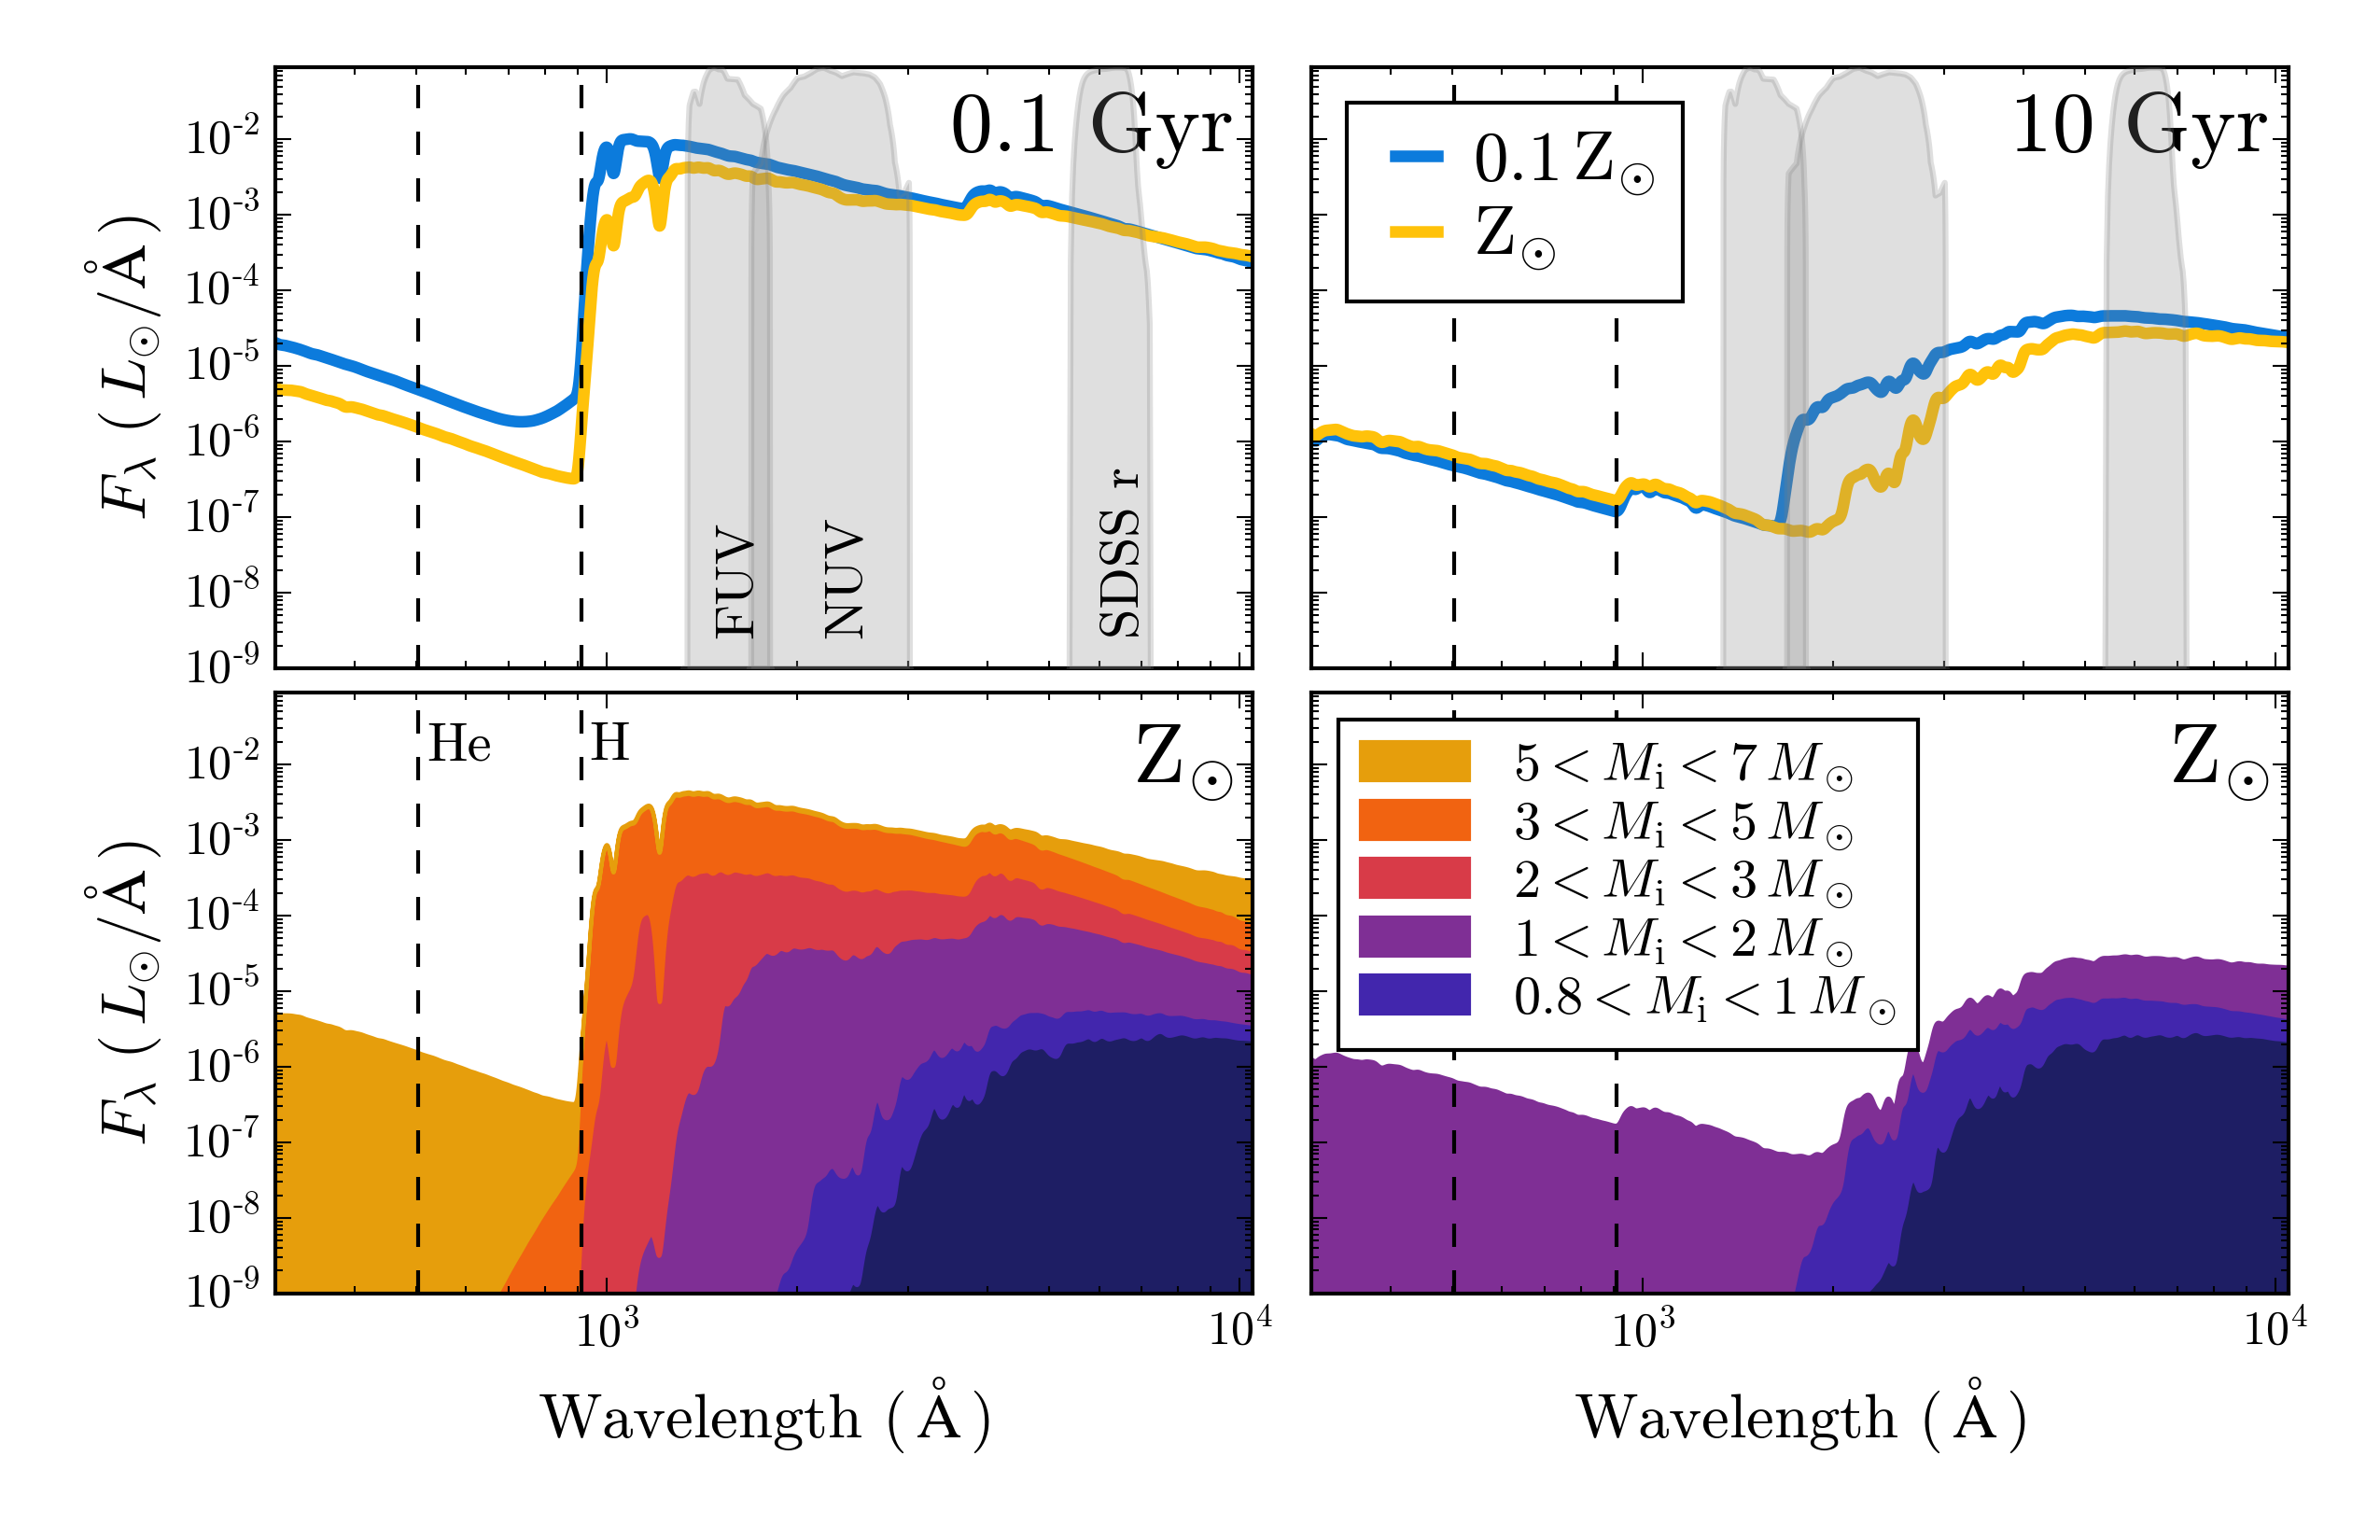
\includegraphics[width=\linewidth]{figs/f1.png}
    \caption{The UV-optical spectrum for an instantaneous burst at 0.1\Gyr (\emph{left}) and 8\Gyr (\emph{right}). In all panels, we overlay the transmission of the GALEX FUV, NUV and SDSS r-band filters, and the dashed lines indicate the ionization energy of helium ($E\geq24.6\,$eV or $\lambda \geq 504\,$\ang) and hydrogen ($E\geq13.6\,$eV or $\lambda \geq 912\,$\ang). \emph{Top:} The total SED at several metallicities, from \logZeq{-2} to 0.5. \emph{Bottom:} For a solar metallicity SSP, the SED is now broken down by stellar mass.}
    \label{fig:ionSpec}
  \end{center}
\end{figure*}
%-------------------------------------------------------

To understand the origin of this UV emission, Fig.~\ref{fig:FracSpec} shows the break down of the spectrum by evolutionary type at 10\% solar (\emph{top}) and solar (\emph{bottom}) metallicity for the 8\Gyr population. We plot the fractional contribution to the total flux from main sequence, red giant branch, horizontal branch, AGB, and post-AGB stars, as designated by the phases tagged in the MIST isochrone tables. The AGB label includes the contribution from both early-AGB and thermally pulsing-AGB (TP-AGB) phases. We omit the WR phase from the plot, as these stars are present for $\lesssim5$\Myr in instantaneous burst populations. At both metallicities the optical light is dominated by main sequence and RGB stars. Even at 8\Gyr, main sequence stars still dominate the GALEX NUV band, while post-AGB stars dominate the GALEX FUV band.

The populations that drive the UV colors will change with metallicity, since metallicity can change the temperature and lifetime of various stellar phases. In the model at 10\% solar metallicity, the hotter main sequence stars contribute a higher fraction of the total flux in the GALEX FUV and NUV filters. At solar metallicity, post-AGB stars are responsible for $\sim98\%$ and $\sim10\%$ of the FUV and NUV flux, respectively. At \logZeq{-1}, the post-AGB contribution decreases to $\sim90\%$ and $\sim1\%$ of the FUV and NUV filters, respectively. In both cases, however, the post-AGB stars are responsible for all of the flux produced at energies sufficient to ionize hydrogen and helium. 
%-------------------------------------------------------
% Fractional contribution by EvType for Z=-1, 0.0
%-------------------------------------------------------
\begin{figure}
  \begin{center}
    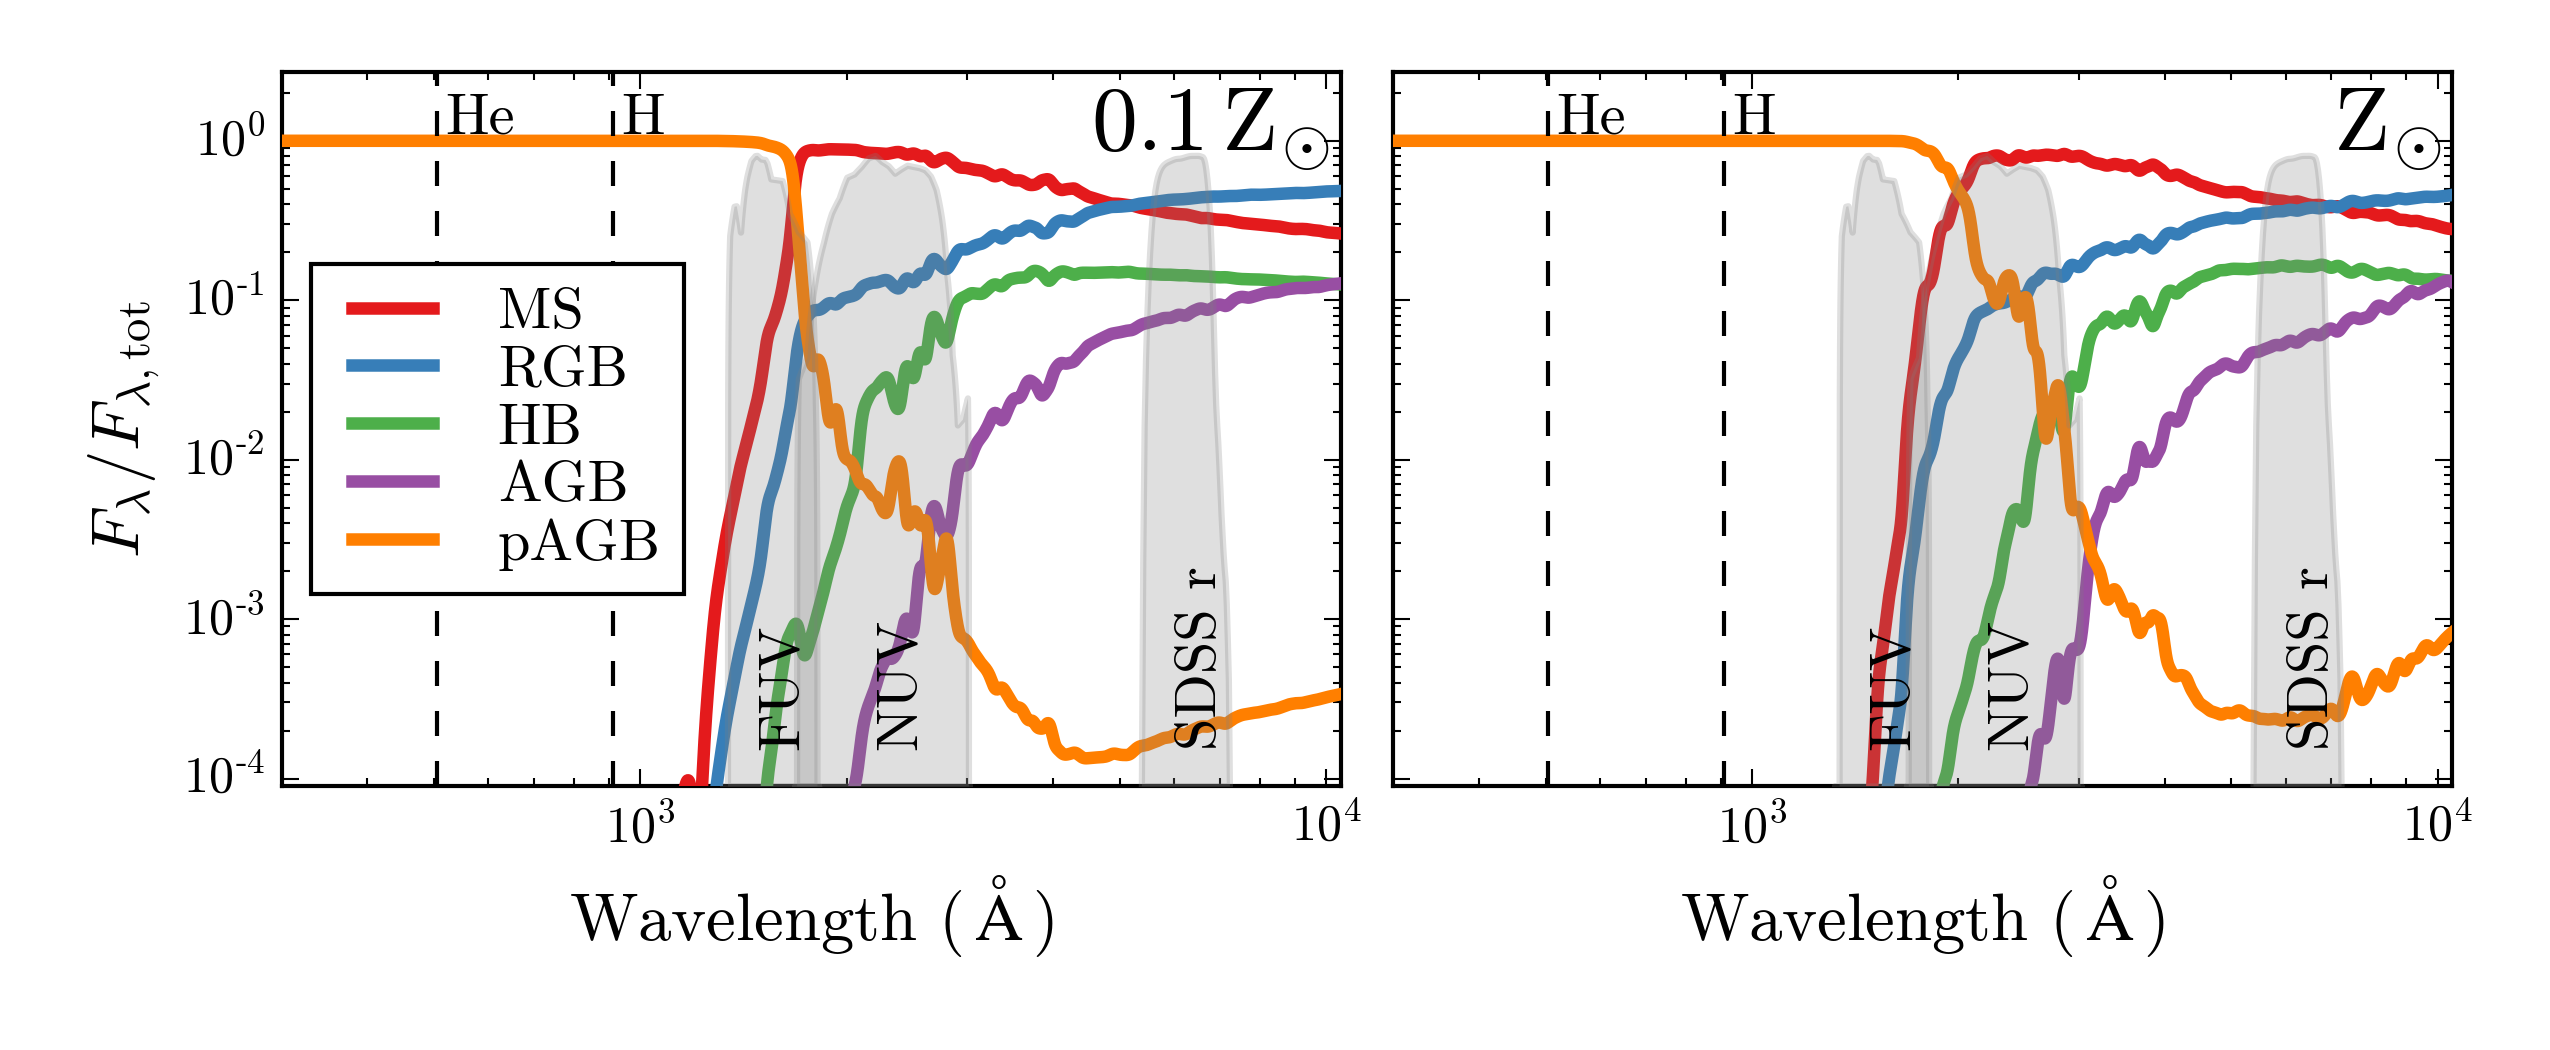
\includegraphics[width=\linewidth]{figs/f2.png}
    \caption{The ionizing spectrum from an 8\Gyr old burst ($\log t=9.9$) at \logZeq{-1} (\emph{top}) and \logZeq{0.0} (\emph{bottom}), showing the fractional contribution of various evolutionary phases to the total SED, including main sequence (MS), red giant branch (RGB), horizontal branch (HB), post-AGB (pAGB), and Wolf-Rayet (WR) stars. The vertical dashed lines show the ionization energy of helium ($E\geq24.6\,$eV or $\lambda \geq 504\,$\ang) and hydrogen ($E\geq13.6\,$eV or $\lambda \geq 912\,$\ang). The grey shaded region shows the transmission of the GALEX FUV, NUV and the SDSS r-band filters.}
    \label{fig:FracSpec}
  \end{center}
\end{figure}
%-------------------------------------------------------

In Fig.~\ref{fig:QF}, we show the ionizing flux from different types of stars as a function of time for instantaneous burst populations. The top panel shows the time evolution of \QH, the number of photons emitted per second that are capable of ionizing hydrogen ($E\geq13.6\,$eV or $\lambda \geq 912\,$\ang) for a 10\% solar (\emph{left}) and solar (\emph{right}) population. The bottom panel shows the time evolution of \QHe, the number of photons emitted per second that are capable of ionizing helium ($E\geq24.6\,$eV or $\lambda \geq 504\,$\ang). For the single-star MIST models, main sequence stars dominate the ionizing photon budget for nearly 100\Myr, with the exception of the brief but intense contribution from Wolf-Rayet stars at 2-4\Myr ($\log t\sim6.5$). The first post-AGB stars appear after a few hundred \Myr. These stars are quite hot and dominate both the hydrogen- and helium-ionizing flux once they appear. At all metallicities in the standard MIST models, post-AGB stars make up more than 95\% of the ionizing flux after $\sim200$\Myr, while HB stars never contribute more than 10\%.
%-------------------------------------------------------
% Time evolution of QH/QHe by EvType for 1/10 solar (left) and solar (right)
%-------------------------------------------------------
\begin{figure*}
  \begin{center}
    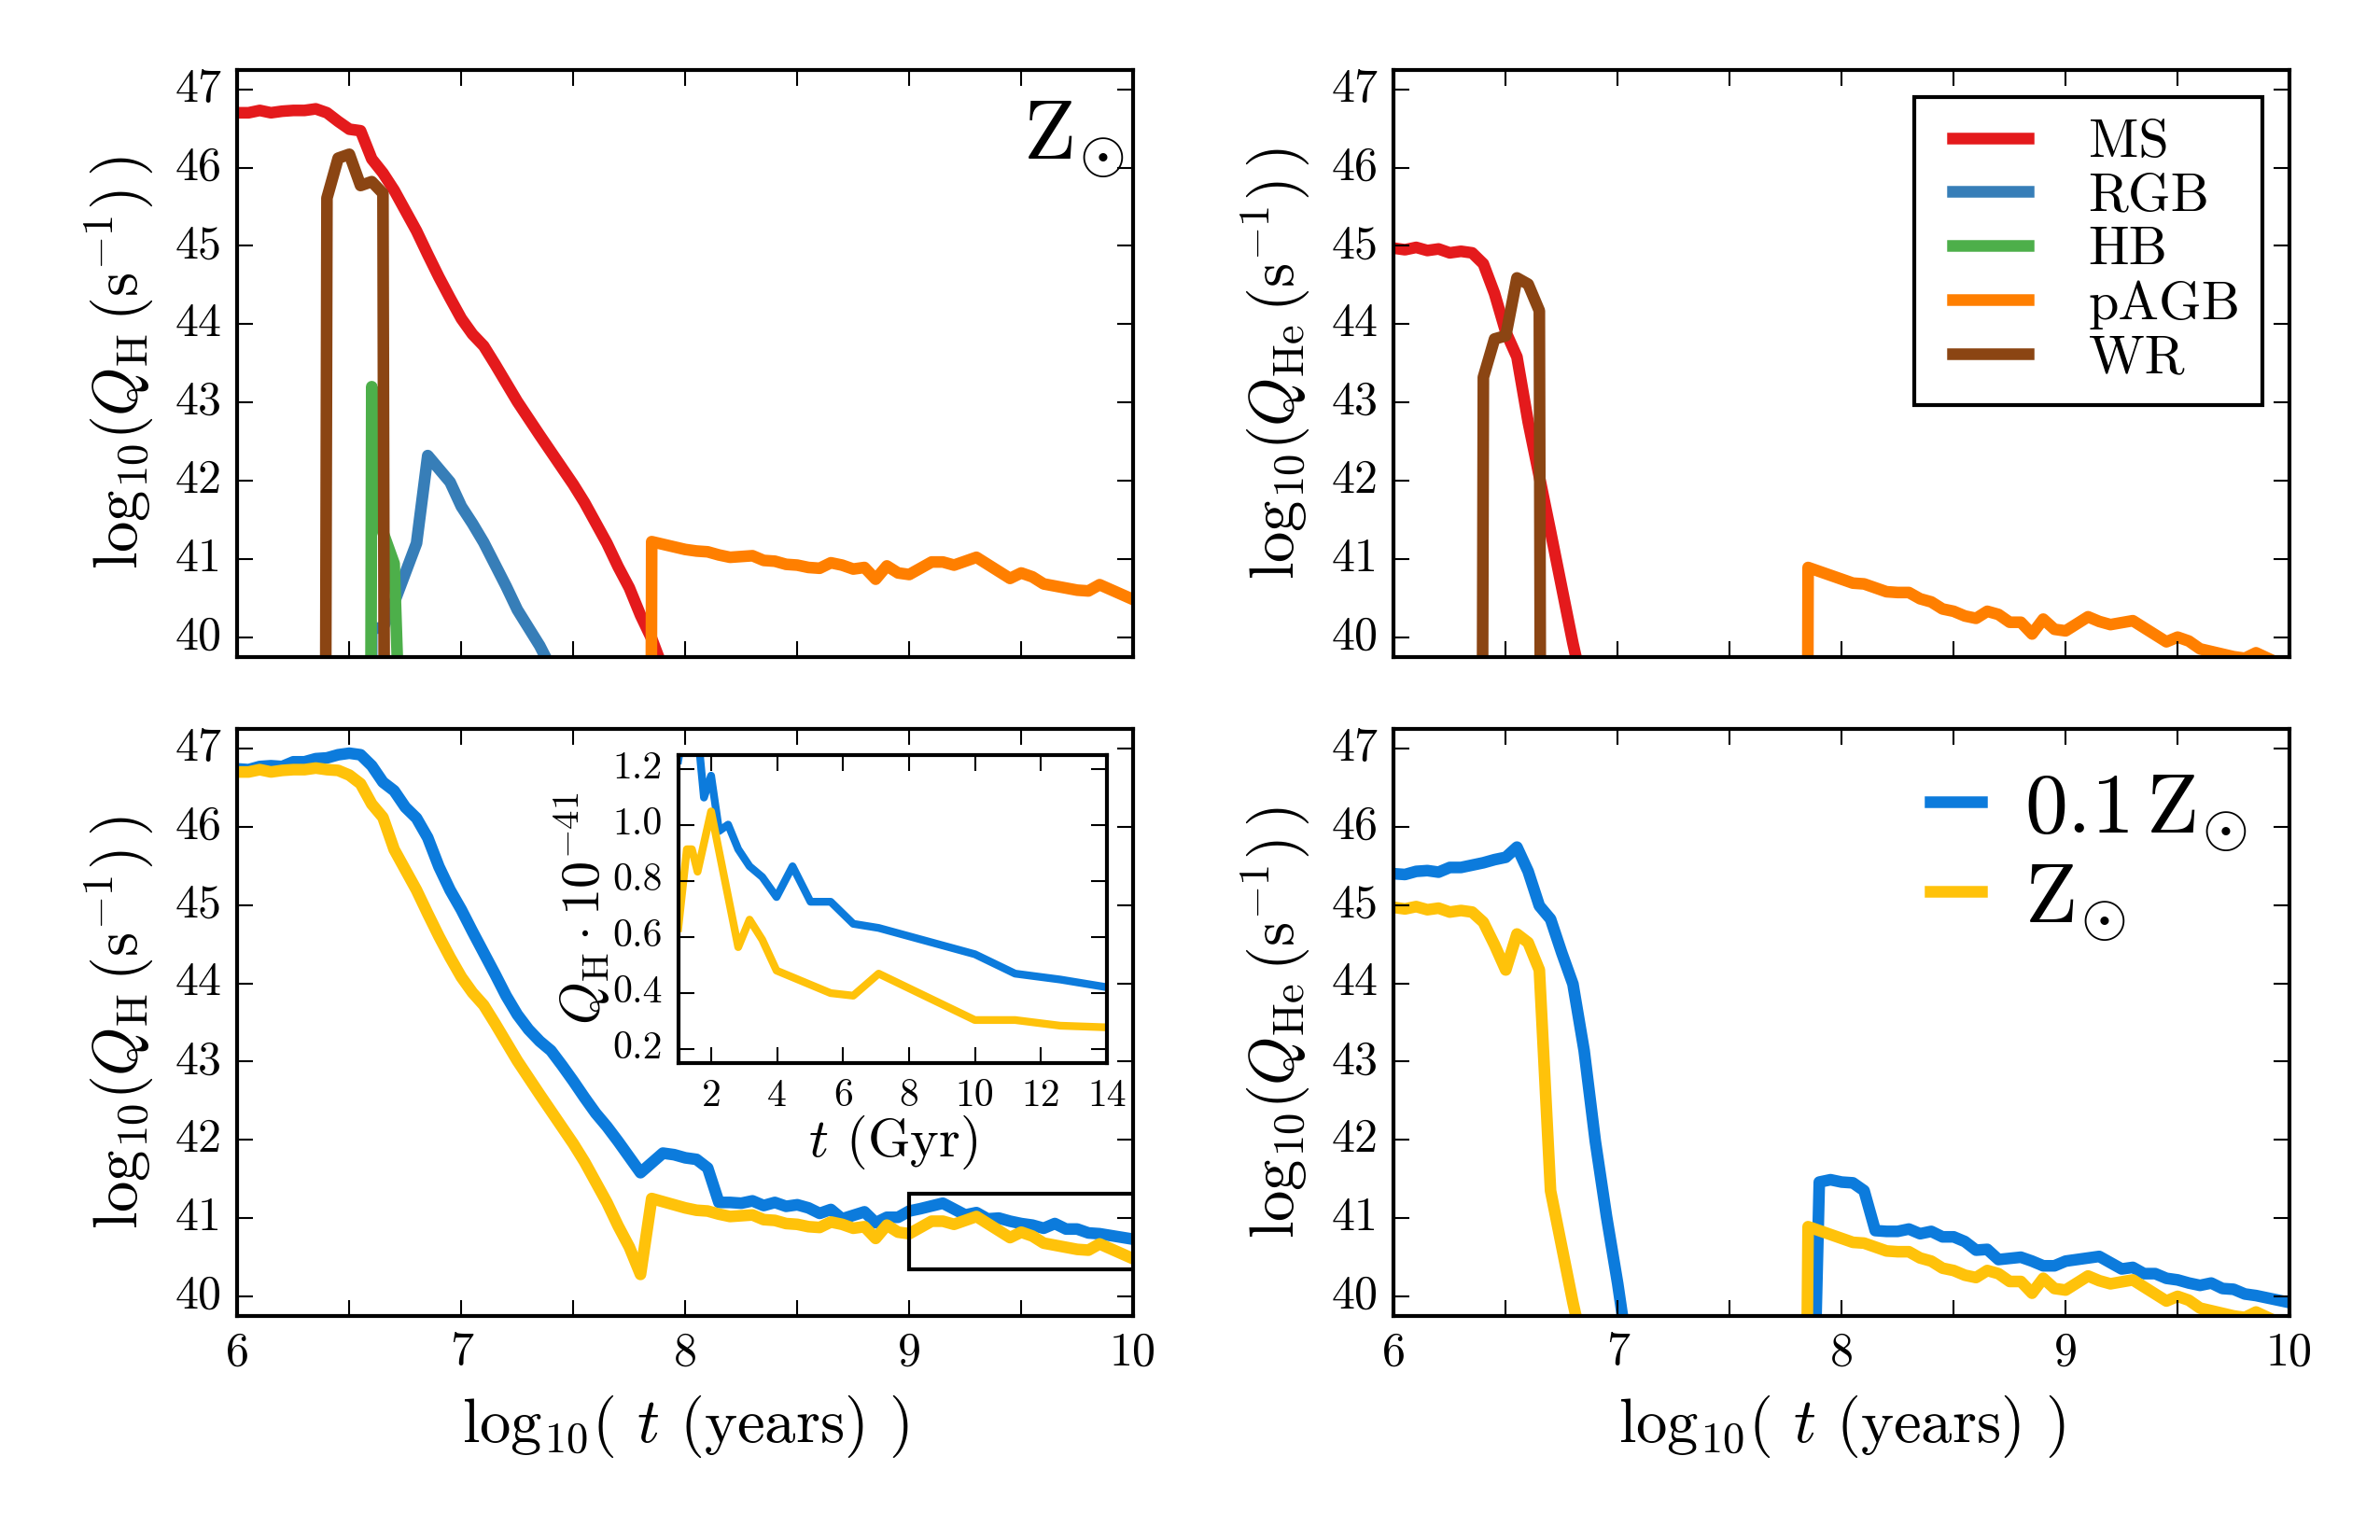
\includegraphics[width=\linewidth]{figs/f3.png}
    \caption{\emph{Top row}: The ionizing photon flux per unit stellar mass for Hydrogen, \QH, as a function of time for different stellar types at 1/10 solar (\emph{left}) and solar metallicity (\emph{right}) for instantaneous burst populations. \emph{Bottom}: The ionizing photon flux per unit stellar mass for Helium, \QHe, as a function of time for different stellar types at 1/10 solar (\emph{left}) and solar metallicity (\emph{right}) for instantaneous burst populations. The evolutionary phases shown include the Main Sequence (MS), Red Giant Branch (RGB), Horizontal Branch (HB), post-AGB (pAGB), and Wolf-Rayet (WR) stars. After the massive main sequence and WR stars have died, post-AGB stars provide the bulk of the ionizing radiation. These stars are hot enough to ionize both hydrogen and helium, but produce ionizing photon rates that are $10^5$ times lower than MS stars, requiring large numbers of stars to produce substantial \ha flux. Binary evolution can potentially extend the initial ionizing phase to $\sim10-15$\Myr.}
    \label{fig:QF}
  \end{center}
\end{figure*}
%-------------------------------------------------------

We show the resulting time evolution of \QH and \QHe for instantaneous bursts in Fig.~\ref{fig:popQs}. As explained, \QH and \QHe decline steadily and by orders of magnitude as young, massive stars evolve off of the main sequence. After 1\Gyr, \QH plateaus as the first post-AGB stars appear, but at a level that is more than $10^5$ times smaller than the initial burst. The evolution of helium ionization is somewhat different. \QHe also declines by orders of magnitude over the first Gyr, however, because post-AGB stars can have temperatures akin to late-O or early-B-type stars (15,000-50,000K), \QHe \emph{rises} after 1\Gyr. The He ionizing photon flux is still $10^5$ times smaller than during the initial burst, however.

For young, massive stars, \QH changes with metallicity, since metal line blanketing in the atmospheres of stars reduces the amount of emergent flux in the UV. The late time evolution of \QH and \QHe is largely independent of metallicity, when post-AGB stars dominate the ionizing flux. The post-AGB models occupy a narrow range of luminosities and the temperature sequence is an aging process rather than a metallicity driven process.


%-------------------------------------------------------
% Total time evolution for QH, QHe at all metallicities
%-------------------------------------------------------
\begin{figure}
  \begin{center}
    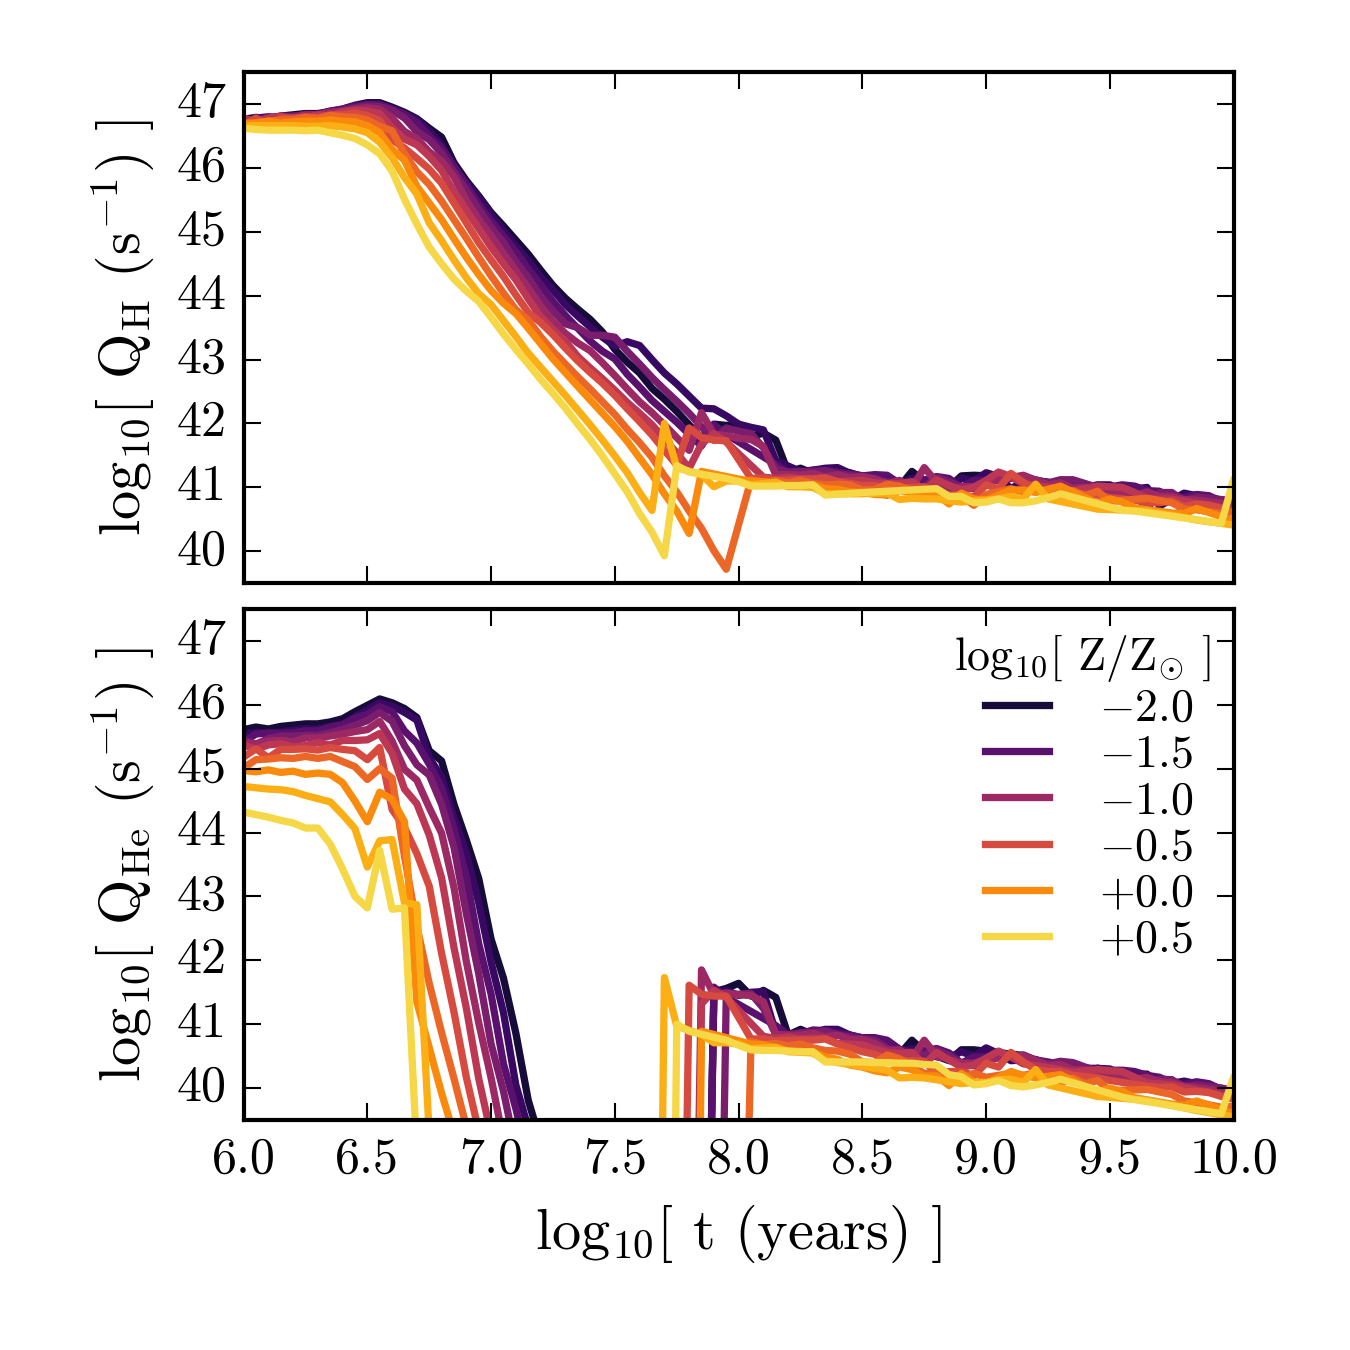
\includegraphics[width=\linewidth]{figs/f4.png}
    \caption{\emph{Top}: The ionizing photon flux per unit stellar mass, \QH, as a function of time for stellar populations with metallicities varying from \logZeq{-2} to \logZeq{0.5}. \emph{Bottom}: The ionizing photon flux per unit stellar mass for Helium, \QHe, as a function of time. For young stars, the metal-poor populations have higher ionizing photon rates and extended main-sequence lifetimes. The bump in \QH at $\log t = 7.8$ seen in populations with metallicities below \logZeq{-0.5} is due to hot horizontal branch stars, which are not hot enough to produce a similar bump in \QHe. The large increase in \QHe after $\log t = 8$ is due to the first onset of post-AGB stars.}
    \label{fig:popQs}
  \end{center}
\end{figure}
%-------------------------------------------------------
%===============================================================================
\subsection{Emission lines from hot evolved stars} \label{sec:stars:emis}

We have used the spectra presented in \S\ref{sec:stars:ion} as the ionizing spectrum input to \Cloudy models. In this section we discuss models run at a range of ionization parameters, $-6<\,$\logU$\,<-3$, typical of LIER-like emission, and assume constant gas phase metallicity, using the solar-like abundances specified in Table~\ref{tab:LIERabd}. The resultant nebular line and continuum spectrum is included as look-up tables within \FSPS.

\subsubsection{Emission line equivalent widths} \label{sec:stars:EW}

To measure \ha equivalent widths from our models, we largely follow the methodology of \citet{Belfiore+2016}, who measured \ha equivalent widths in LIER galaxies with the Mapping Nearby Galaxies at APO survey \citep[MaNGA; ][]{Bundy+2015}. In broad terms, the process involves subtracting the Balmer absorption due to the best-fit stellar continuum, and then fitting the residual emission with a Gaussian. In practice, our methodology differs from this slightly, since we are measuring model equivalent widths with a perfect knowledge of the underlying stellar continuum.

In detail, the process is as follows. We generate two spectra with \FSPS, one that includes nebular emission lines and one that does not. We use the ``non-emission'' spectrum as the best-fit stellar continuum. \FSPS returns $\mathcal{F}_{\lambda}$ in \Lsun/\ang, which we convert to cgs units (erg/s/cm$^{-2}$/\ang) by arbitrarily assuming a mass of $6 \times 10^{10}$\Msun, typical of a massive early-type galaxy, and a distance of 10$\,$Mpc. For both spectra, we scale the flux to the median flux in the continuum spectrum as measured in the 6000-6200\ang range and subtract the continuum spectrum from the emission spectrum. 

We fit the resultant scaled emission-line-only spectrum with \texttt{scipy.optimize.curvefit} \citep{SciPy} using a 3-parameter Gaussian function of the form:
\begin{equation}
    f(x) = a \cdot \exp \left( \frac{-(x-b)^2}{2c^2} \right),
\end{equation}
such that the integrated flux in the Gaussian is simply $\sqrt{2\pi} \cdot ac$ and an equivalent width with units of \ang.

In Fig.~\ref{fig:EW} we show the \ha EW as a function of time for single-aged populations at different metallicities after an initial burst. \ha EWs are strongest at young ages, when hot, young stars produce copious amounts of ionizing radiation and strong \ha emission is on top of a weaker optical stellar continuum. At the same age, \ha EWs for metal-poor populations are larger, due to the harder ionizing spectra of metal-poor stars. The metal-poor populations also have longer main-sequence lifetimes, producing larger \ha EWs for several \Myr longer than the solar-metallicity population.

In general, the \ha equivalent widths in Fig.~\ref{fig:EW} decline with time until ${\sim}1$\Gyr, where EWs increase again due to the onset of the post-AGB phase. After $\log t \sim 9$, equivalent widths increase as the population of stars in the post-AGB phase grows. The elevated \ha EWs seen in populations with metallicities below \logZeq{-0.5} just before $\log t \sim 8$ reflect the rising contribution from hot horizontal branch stars. As seen in Fig.~\ref{fig:QF}, these stars are important between 10 and 100\Myr. The effect is stronger with decreasing metallicity, and the lowest metallicity populations (\logZeq{-2}) produce \ha EWs an order of magnitude larger than the solar-metallicity populations at the same age. 

The grey shaded region in Fig.~\ref{fig:EW} shows the range of EWs measured in typical LIER-like galaxies, of order 0.1-6\ang. At late times ($\log t \gtrsim 9$), our models produce equivalent widths consistent with observed LIERs. This is the first successful prediction for emission line equivalent widths using stellar models where the post-AGB stars have been fully modeled from the main sequence through the post-AGB phase.


%-------------------------------------------------------
% Ha EW time evolution
%-------------------------------------------------------
\begin{figure*}
  \begin{center}
    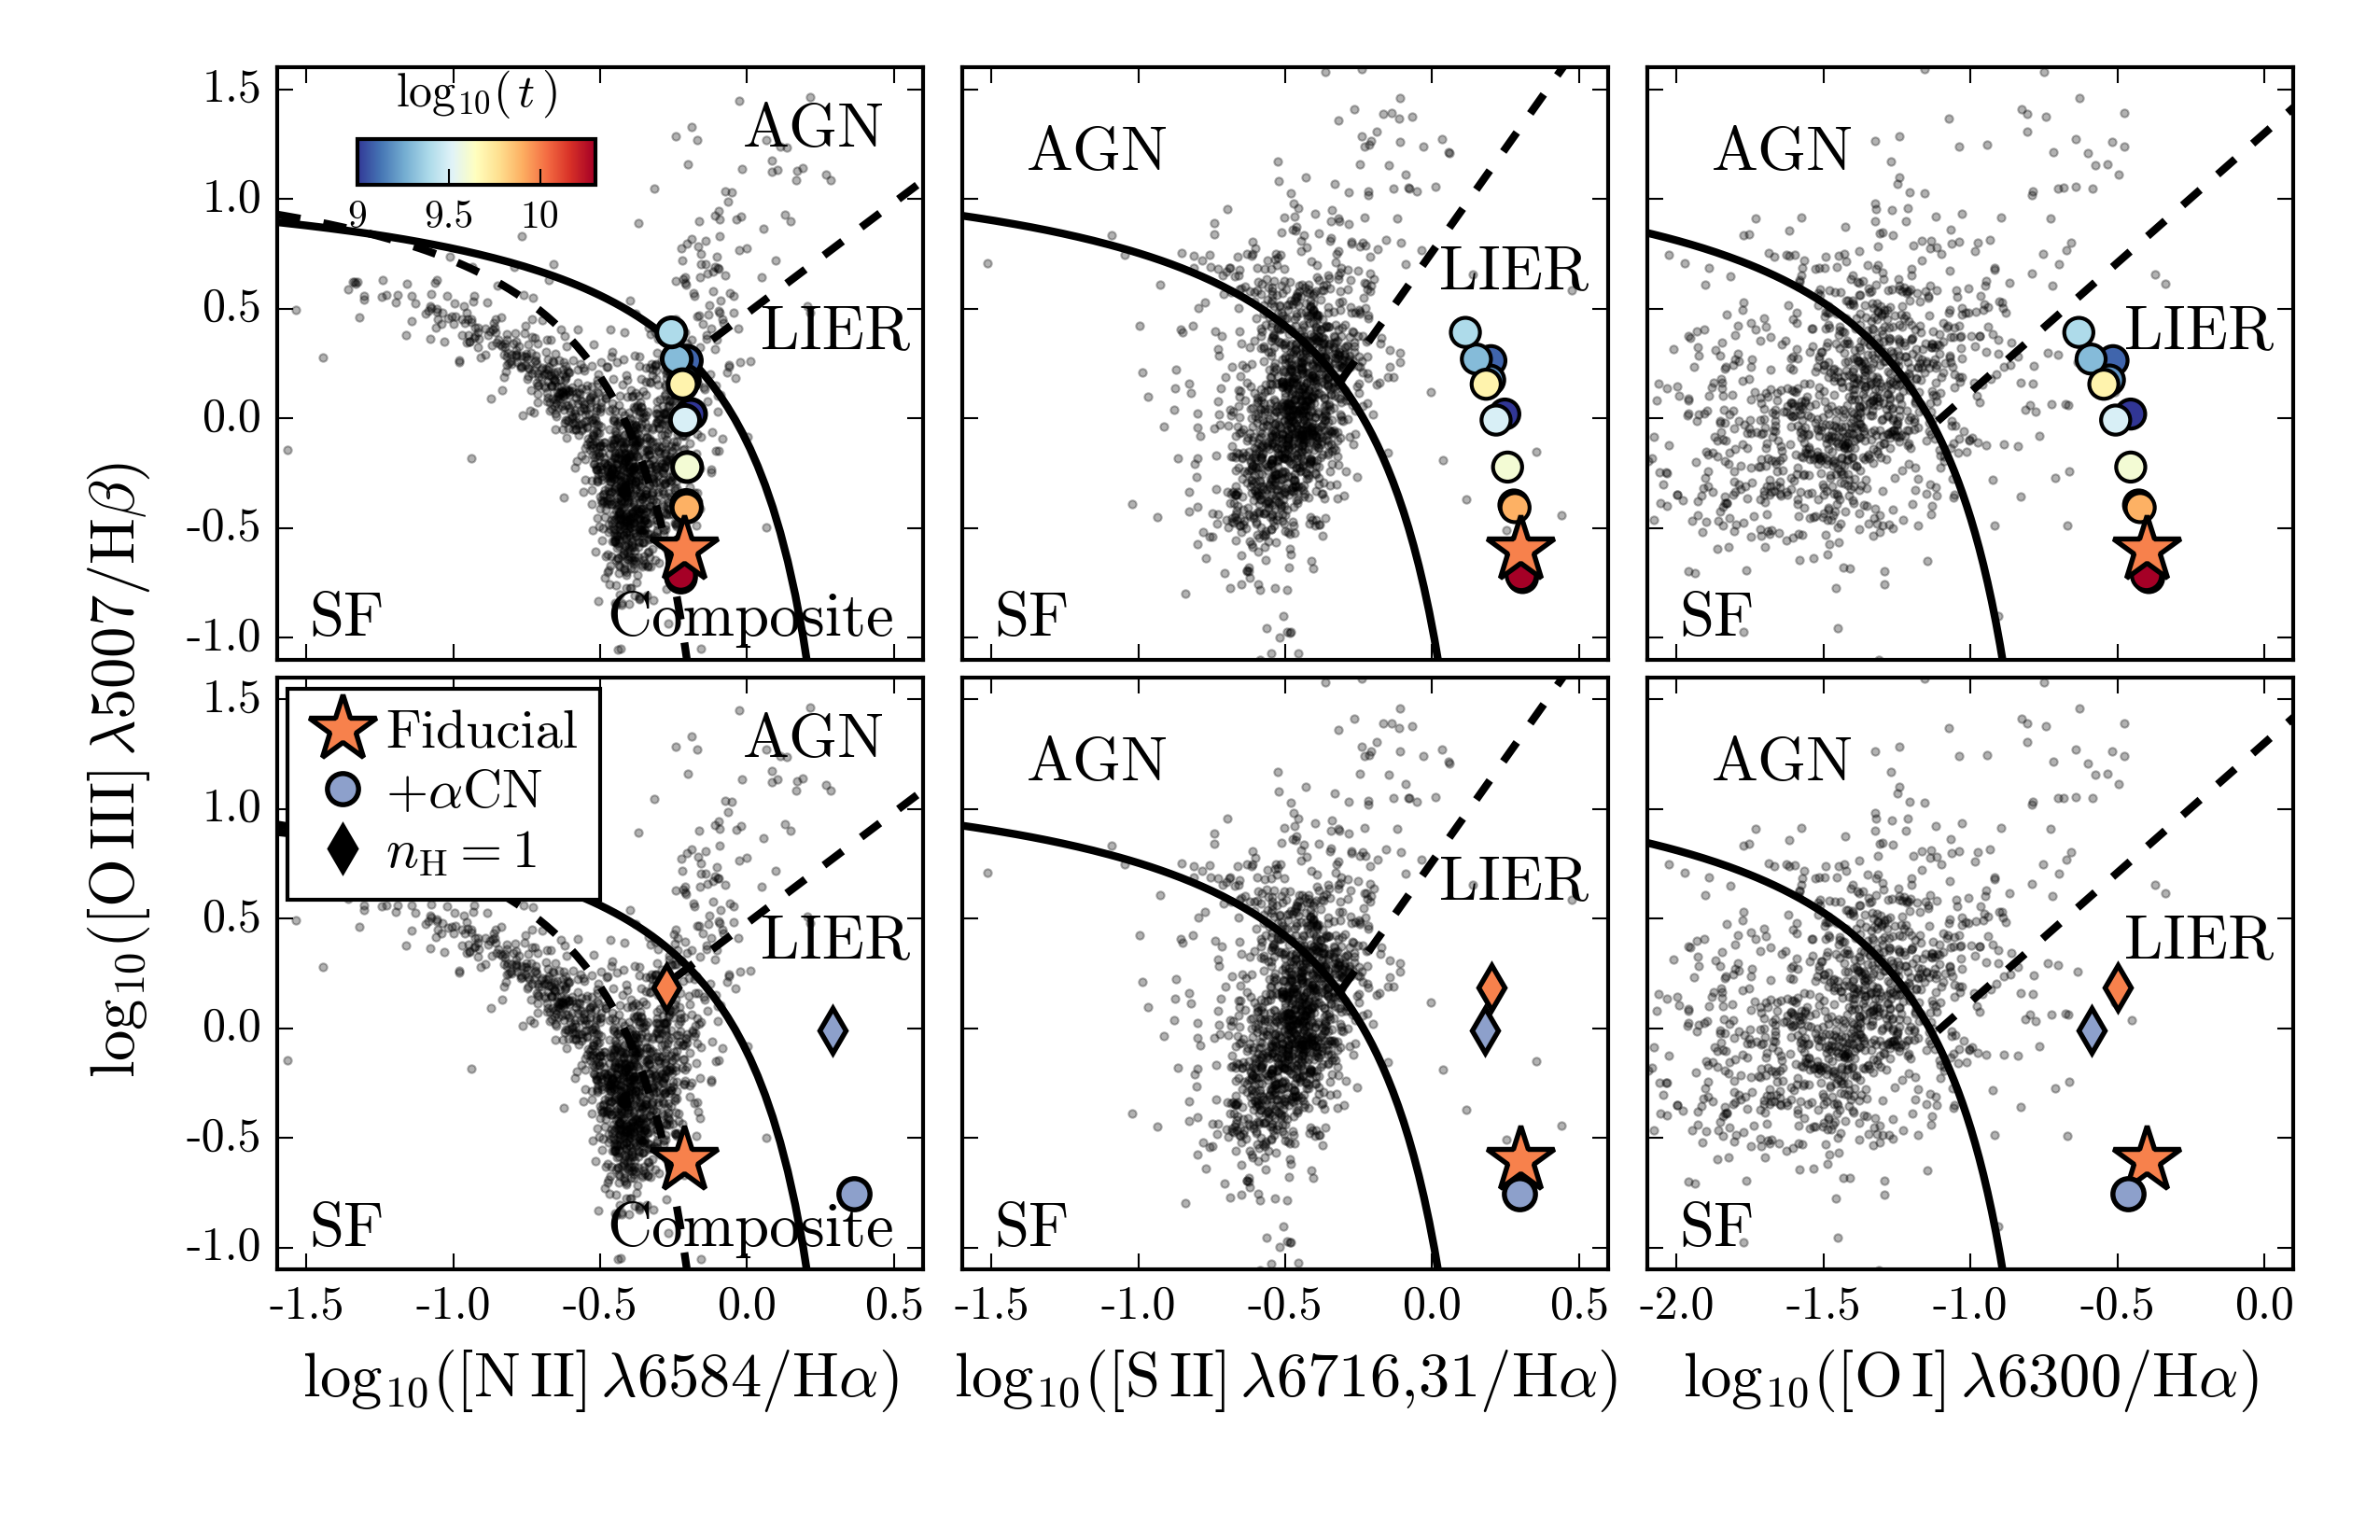
\includegraphics[width=\linewidth]{figs/f5.png}
    \caption{The time evolution of \ha equivalent widths for single-aged populations with \logUeq{-4}, a reproduction of Figure 2 from \citet{Belfiore+2016}. Nebular emission is strongest at young ages, and \ha equivalent widths decline quickly after the first few Myr. The grey shaded region highlights \ha EWs observed in typical LIER-like galaxies, of order $0.1-3\,$\ang. The post-AGB stars are responsible for the increase in \ha EW seen at $\log t \gtrsim 9$.}
    \label{fig:EW}
  \end{center}
\end{figure*}
%-------------------------------------------------------

\subsubsection{Emission line ratios} \label{sec:stars:ratios}

In Fig.~\ref{fig:BPT1} we show the standard BPT diagram, a widely-used diagnostic that generally separates objects with different ionization states. We show the line ratios from our post-AGB model, for an 8\Gyr instantaneous burst at a range of stellar metallicities, with the gas phase metallicity fixed at solar metallicity. The post-AGB models produce emission line ratios in good agreement with the LIER/LINER region of the diagram. Models with ionization parameters between \logUeq{-5} and \logUeq{-3} easily match line ratios observed in LIER-like galaxies.

From Fig.~\ref{fig:ionSpec} we should not be surprised that there is little difference between models with different stellar metallicities, since the post-AGB stars producing the ionizing radiation have very similar colors. The ionizing spectra have similar hardness, producing gas with similar ionization states and thus similar emission line ratios. While stellar metallicity has little effect on the emission line ratios, it does change the equivalent widths, as seen in Figs.~\ref{fig:EW} \& \ref{fig:EWtau}, but largely through the properties of the continuum, rather than the emission lines.

In Figs.~\ref{fig:BPT2} \& \ref{fig:BPT3} we show the post-AGB model on two additional emission line diagnostic diagrams. The \sii/\ha (Fig.~\ref{fig:BPT2}) and \oi/\ha diagrams (Fig.~\ref{fig:BPT3}) have been highlighted as LIER diagnostics, since they make use of low-ionization lines. In both the \sii/\ha diagram (\emph{middle}) and \oi/\ha diagram (\emph{right}), the models produce line ratios well above the \citet{Kewley+2006} classification line for star-forming galaxies. The post-AGB star models occupy a region distinct from star forming galaxies and consistent with line ratios observed in LIER-like galaxies.

%In summary, Figures~\ref{fig:EW} - \ref{fig:BPT} indicate that our models produce emission line ratios that agree well with those observed in LIER-like galaxies, with no fine tuning needed to produce acceptable models. % Their optical colors and line indices are consistent with ETGs and simultaneously produce emission line equivalent widths and emission line ratios observed in LIER-like galaxies. Moreover, consistent models are produced for a wide range of possible SFHs and ages, with only weak dependencies on metallicity and ionization parameter.
%Given how robust the predictions are, it's probably worth thinking about why every galaxy wouldn't show LIER emission.

%-------------------------------------------------------
% Diagnostic diagrams
%-------------------------------------------------------
\begin{figure}
  \begin{center}
    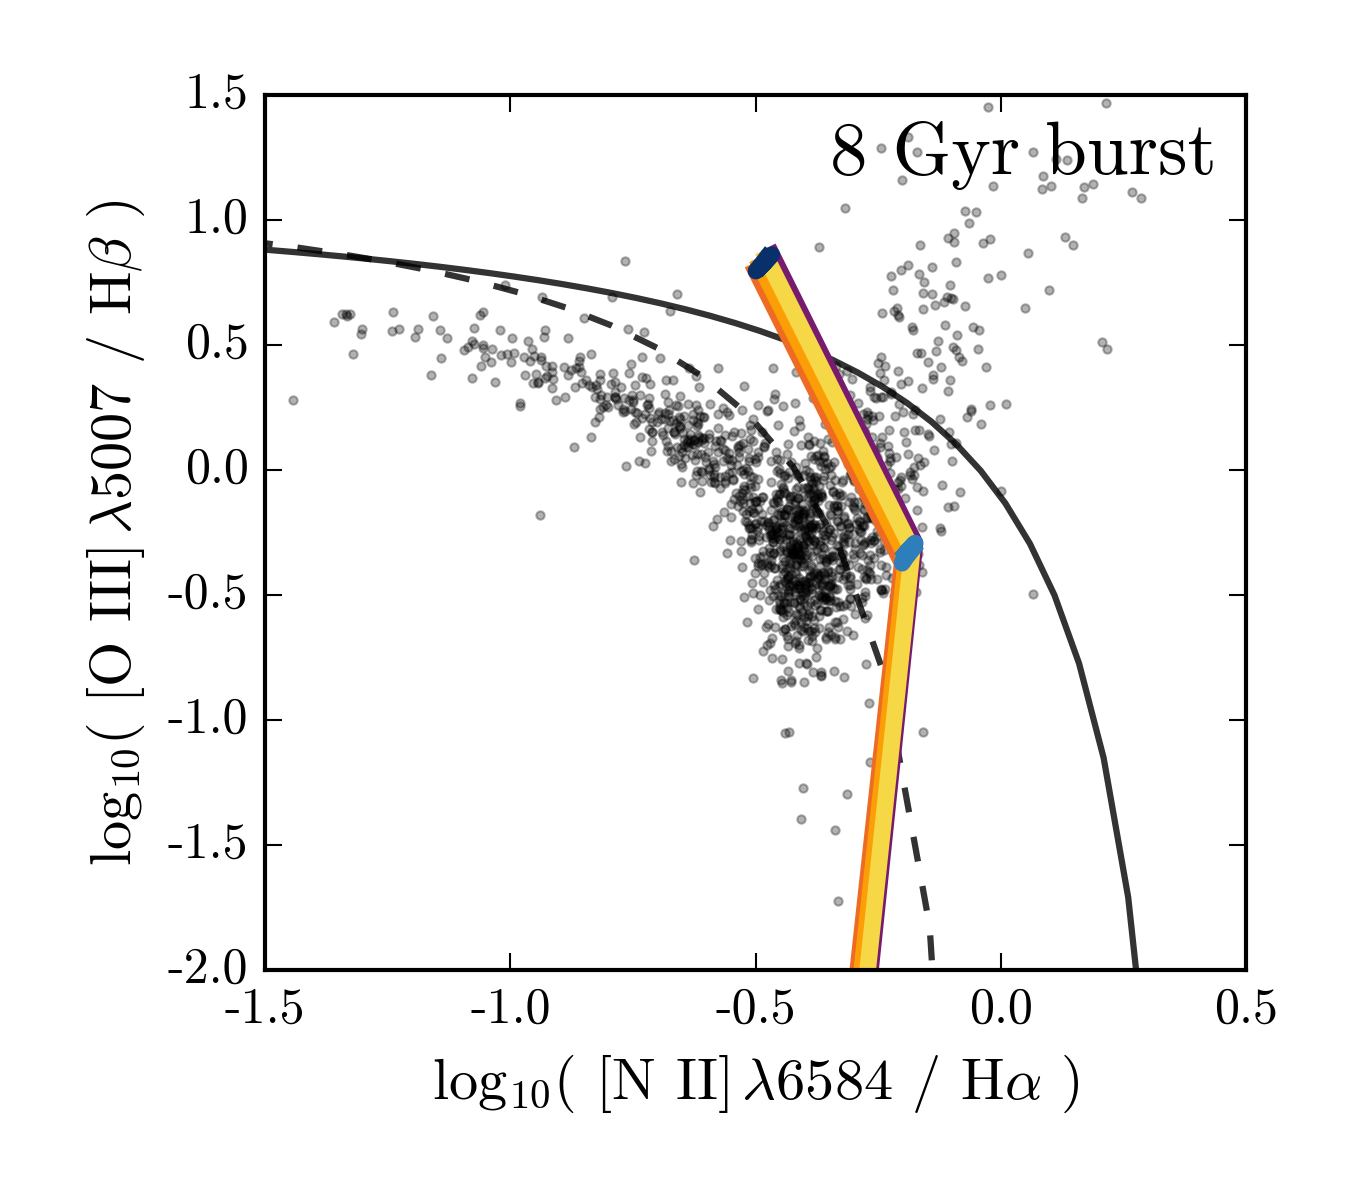
\includegraphics[width=\linewidth]{figs/f6.png}
    \caption{The classic BPT diagram. The models shown are for instantaneous bursts at 8\Gyr. The stellar metallicities vary from \logZeq{-2} to 0.5, but the gas phase metallicity is held constant with solar-like abundances. The ionization parameter is varied from \logUeq{-6} to \logUeq{-3}, typical for LIER-like emission. The dashed line from \citet{Kauffmann+2003b} separates pure star forming galaxies, while the solid line from \citet{Kewley+2001} shows the limit for extreme starbursts. The black points are a selection of SDSS galaxies.}
    \label{fig:BPT1}
  \end{center}
\end{figure}
%-------------------------------------------------------
\begin{figure}
  \begin{center}
    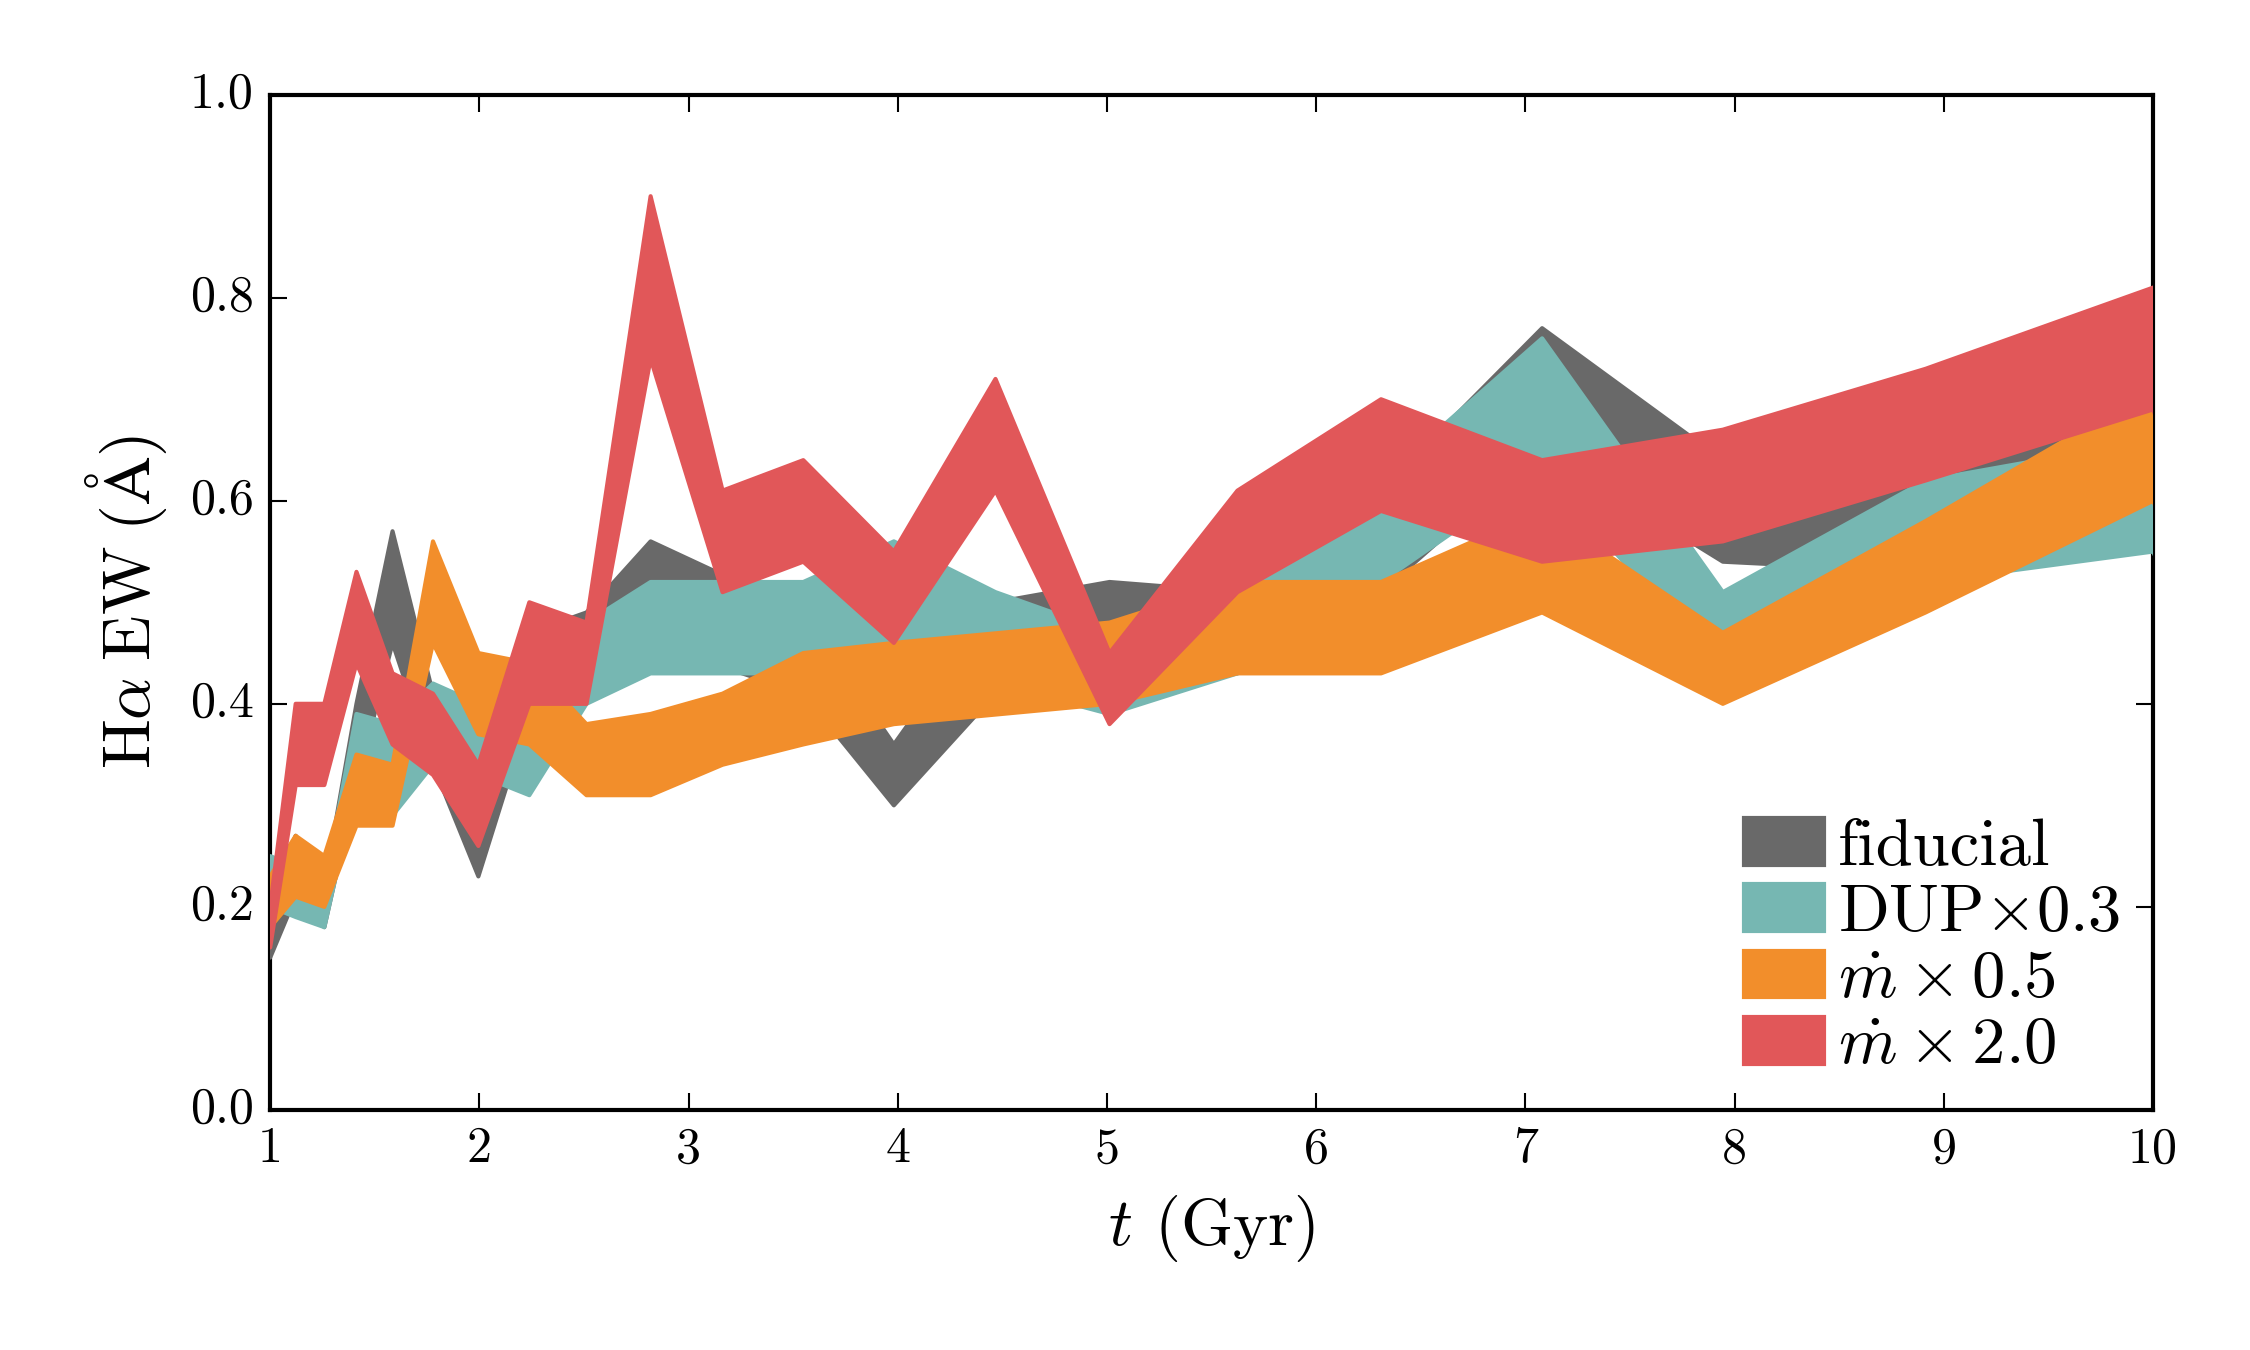
\includegraphics[width=\linewidth]{figs/f7.png}
    \caption{The \sii/\ha \vs \oiii/\hb emission line ratio diagnostic diagram. The models shown are for instantaneous bursts at 8\Gyr. The stellar metallicities vary from \logZeq{-2} to 0.5, but the gas phase metallicity is held constant with solar-like abundances. The ionization parameter is varied from \logUeq{-6} to \logUeq{-3}, typical for LIER-like emission. The solid black line shows the \citet{Kewley+2006} classification for star-forming galaxies. The black points are a selection of SDSS galaxies.}
    \label{fig:BPT2}
  \end{center}
\end{figure}
%-------------------------------------------------------
\begin{figure}
  \begin{center}
    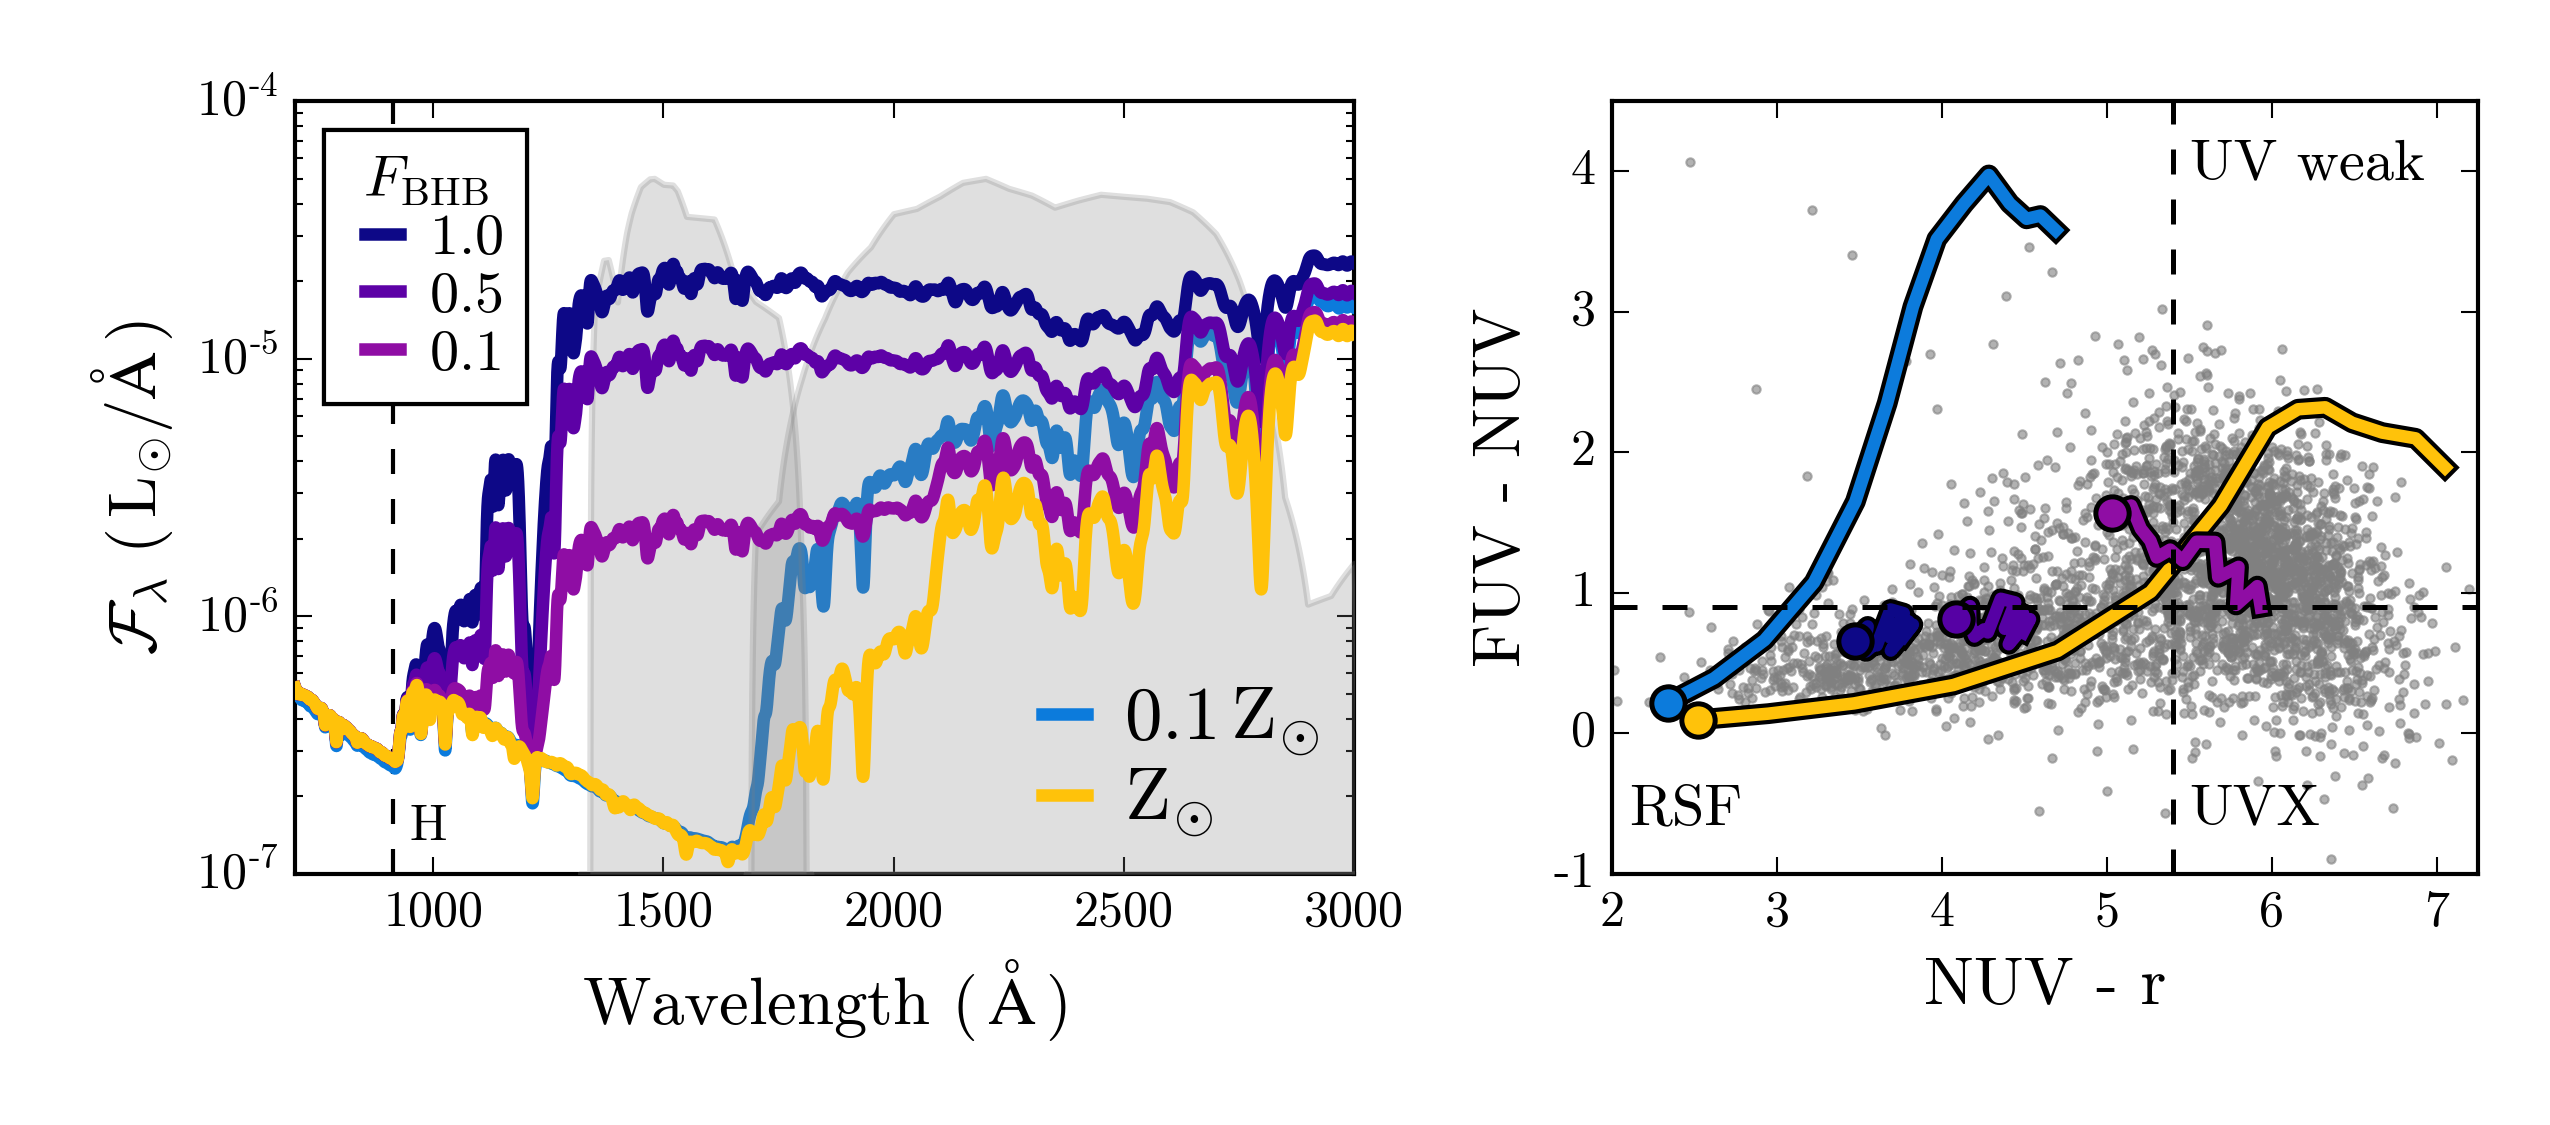
\includegraphics[width=\linewidth]{figs/f8.png}
    \caption{The \oi/\ha \vs O$_{32}$ emission line ratio diagnostic diagram. The models shown are for instantaneous bursts at 8\Gyr. The stellar metallicities vary from \logZeq{-2} to 0.5, but the gas phase metallicity is held constant with solar-like abundances. The ionization parameter is varied from \logUeq{-6} to \logUeq{-3}, typical for LIER-like emission. The solid black line shows the \citet{Kewley+2006} classification for star-forming galaxies. The black points are a selection of SDSS galaxies.}
    \label{fig:BPT3}
  \end{center}
\end{figure}
%-------------------------------------------------------

\section{The underlying stellar continuum} \label{sec:stars:continuum}

For young stellar populations in \hii regions, it is typical to measure \ha fluxes, since these can be tied directly to the mass of recently formed stars. For old stellar populations it is more typical to measure the flux of \ha relative to the continuum using an equivalent width (EW), which partially removes the dependence on stellar mass. The equivalent width of \ha, however, will depend on the strength of \ha \emph{and} the strength of the underlying stellar continuum at optical wavelengths. Making predictions of \ha EWs in old populations therefore requires the self-consistent stellar and nebular models we developed in \citet{Byler+2017}. In this section, we demonstrate that our models have sensible optical colors and absorption lines.

Although it is an oversimplification to model early-type galaxies as a single age, single metallicity population, it is not always an inappropriate representation. In this section, we first demonstrate that instantaneous bursts adequately reproduce observed properties of the ETG population. We then extend the analysis to include more realistic SFHs, with a delayed-$\tau$ model of the form:
\begin{equation}
    \mathrm{SFR}(t) = t \exp (-t/\tau),
\end{equation}
for $\tau = $0.1, 0.5, and 1.0\Gyr and total stellar mass between $10^{10}$ and $10^{11}$\Msun \citep{Thomas+2005, Choi+2014}.

\subsection{Optical colors} \label{sec:stars:continuum:colors}

In Fig.~\ref{fig:optCols} we show the SDSS $u-r$ \vs $r-z$ color-color diagram for our models at a range of ages and metallicities, for stellar-only models (\emph{bottom row}) and stellar+nebular emission models (\emph{top row}, assuming \logUeq{-4}). The $u-r$ \vs $r-z$ diagram has proven to be an efficient means of selecting quiescent, red-sequence ETGs. The \citet{Holden+2012} boundary for selecting quiescent ETGs is indicated with the black dotted line; the \citet{McIntosh+2014} extension for ``recently quenched'' ETGs is shown with the black solid line. In general, the inclusion of nebular emission has little affect on the optical colors. For instantaneous bursts (\emph{left column}), models with metallicities richer than \logZeq{-1} and ages older than $\sim2$\Gyr have optical colors that are appropriate for the ETG population.

Columns two and three of Fig.~\ref{fig:optCols} show the same color-color diagrams for the delayed-$\tau$ models, for $\tau = 0.5$ and 1.0\Gyr, respectively. The models with $\tau=0.1$\Gyr are essentially indistinguishable from the instantaneous bursts, and are thus ommitted from Fig.~\ref{fig:optCols}. The $\tau=0.5$\Gyr models show qualitatively similar behavior to the instantaneous bursts. The $\tau=1$\Gyr models are much bluer than the instantaneous bursts, and only the most metal rich models produce colors consistent with the red, quiescent galaxy population.

%-------------------------------------------------------
% Optical Colors
%-------------------------------------------------------
\begin{figure*}
  \begin{center}
    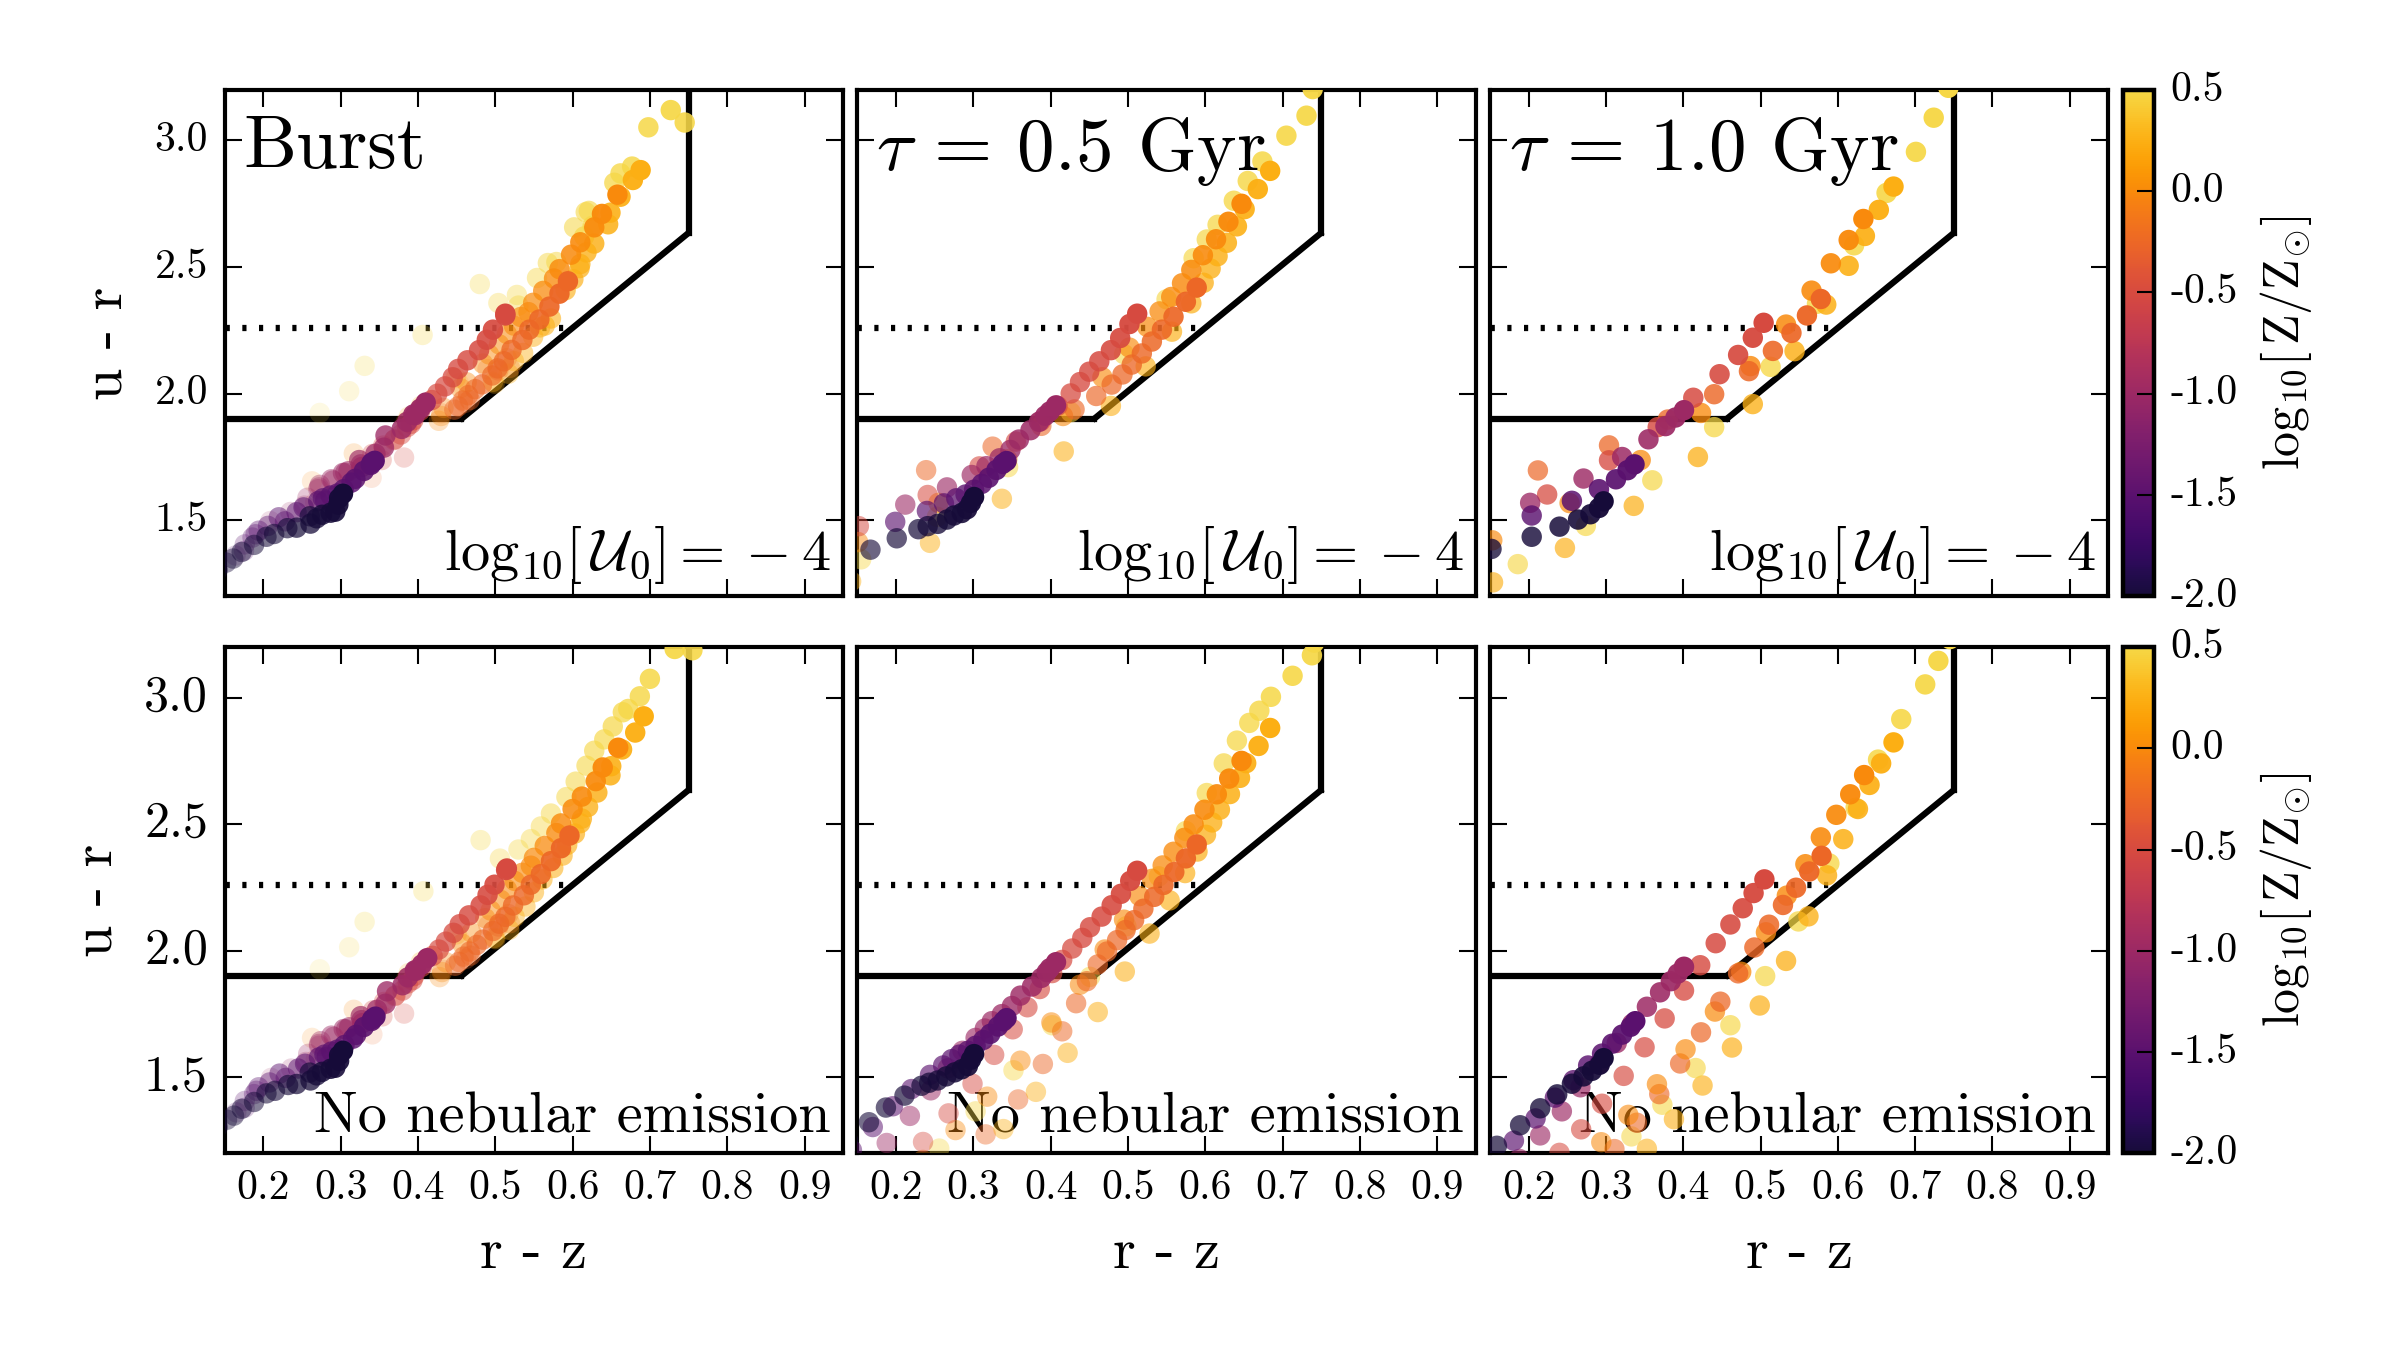
\includegraphics[width=\linewidth]{figs/f9.png}
    \caption{Optical color-color diagram for stellar populations using a delayed$-\tau$ model SFH, with $\tau=0.0$\Gyr (instantaneous burst, \emph{left}), $\tau=0.1$\Gyr (\emph{middle}), and $\tau=0.5$\Gyr (\emph{right}). The top row shows models that include nebular emission, with \logUeq{-4} while the bottom row shows models that do not include nebular emission. Models with ages between 1 and 13\Gyr are plotted, color-coded by metallicity. Age is indicated by the transparency of the points, with the 13\Gyr model points fully opaque. The SDSS $u-r$ \vs r-z colors efficiently separate blue, star-forming galaxies from quiescent, red galaxies. The black line selects ETGs from \citet{Holden+2012}, revised by \citet{McIntosh+2014} to include recently quenched ETGs. The models used in this work have optical colors representative of the general ETG population.}
    \label{fig:optCols}
  \end{center}
\end{figure*}
%-------------------------------------------------------

\subsection{Lick indices} \label{sec:stars:continuum:lick}

The Lick/IDS line strength system \citep{Worthey+1994, Trager+2000} leverages specific spectral features in the optical spectrum that correlate with the age and metallicity of a stellar population. For elliptical galaxies with old stellar populations, stars with initial masses between 1 and 2\Msun dominate both the optical spectrum and the ionizing radiation responsible for LIER-like emission. In this section, we show that our models with nebular emission still produce Lick indices consistent with the general ETG population.

We use Lick definitions from \citet{Vazdekis+2010}. We compare our models to the \hb Lick index and the [MgFe] index, a combination of several Lick indices (\texttt{Mg\_b}, \texttt{Fe5270}, and \texttt{Fe5335}) which is sensitive to metallicity, where higher metallicity populations produce larger values of [MgFe]. The [MgFe] index is also relatively insensitive to $\alpha-$abundance enhancements. To calculate [MgFe], we use the definition from \citet{Galleti+2009}:
\begin{equation}
    [\mathrm{MgFe}] = \sqrt{\texttt{Mg\_b} \times \frac{\texttt{Fe5270} + \texttt{Fe5335}}{2}}.
\end{equation}

In Fig.~\ref{fig:LickMgFe} we show the [MgFe] index compared to the optical SDSS $g-r$ color for our ETG models at different metallicities. As in Fig.~\ref{fig:optCols}, the bottom row shows models without nebular emission, while the top row shows models that include both nebular line and continuum emission, assuming \logUeq{-4}, typical for LIER-like galaxies. Each column shows a different delayed$-\tau$ model, from $\tau=0$\Gyr (instantaneous burst, \emph{left column}) to $\tau=1$\Gyr (\emph{right column}). The grey shaded region indicates the location of elliptical galaxies and ancient, massive, globular clusters (GCs) from \citet{Schombert+2016}.

Our models produce reasonable [MgFe] values, consistent with the low-metallicity GCs and the more metal-rich ETGs. For the $\tau=1$\Gyr model, the extended SF changes the $g-r$ colors significantly until $\sim5$\Gyr, after which the [MgFe] and $g-r$ colors are consistent with the observed ETGs. The [MgFe] indices do not cover spectral regions with any strong nebular emission lines, thus, the models with and without emission are very similar for models at late ages.

In Fig.~\ref{fig:LickHb} we show the age-sensitive \hb Lick index compared to the optical SDSS $g-r$ color in the same style as Fig.~\ref{fig:LickMgFe}. The \hb index is a well-known age-indicator, decreasing as the stellar population ages. The ETGs and GCs from \citet{Schombert+2016} have \hb between 0 and 4\ang, with \hb decreasing as the $g-r$ color gets redder. Our models with and without emission show similar behavior, with high values and blue colors for young models and low \hb combined with redder colors for models over a few Gyr. Models with ages between $2-13$\Gyr are best matched to the ETG and GC data, with lower metallicities for the GCs and higher metallicities for the ETGs. The models with nebular emission show slightly modified \hb values and colors, though overall still consistent with the data. In the models that include emission, \hb emission causes the \hb index to decreases rapidly while the $g-r$ color stays the same.

In what follows, we will largely restrict our analysis of emission lines and UV emission to the subset of models that are also consistent with the observed properties of ETGs in Figures~\ref{fig:optCols} - \ref{fig:LickHb}.

%-------------------------------------------------------
% optical colors
%-------------------------------------------------------
\begin{figure*}
  \begin{center}
    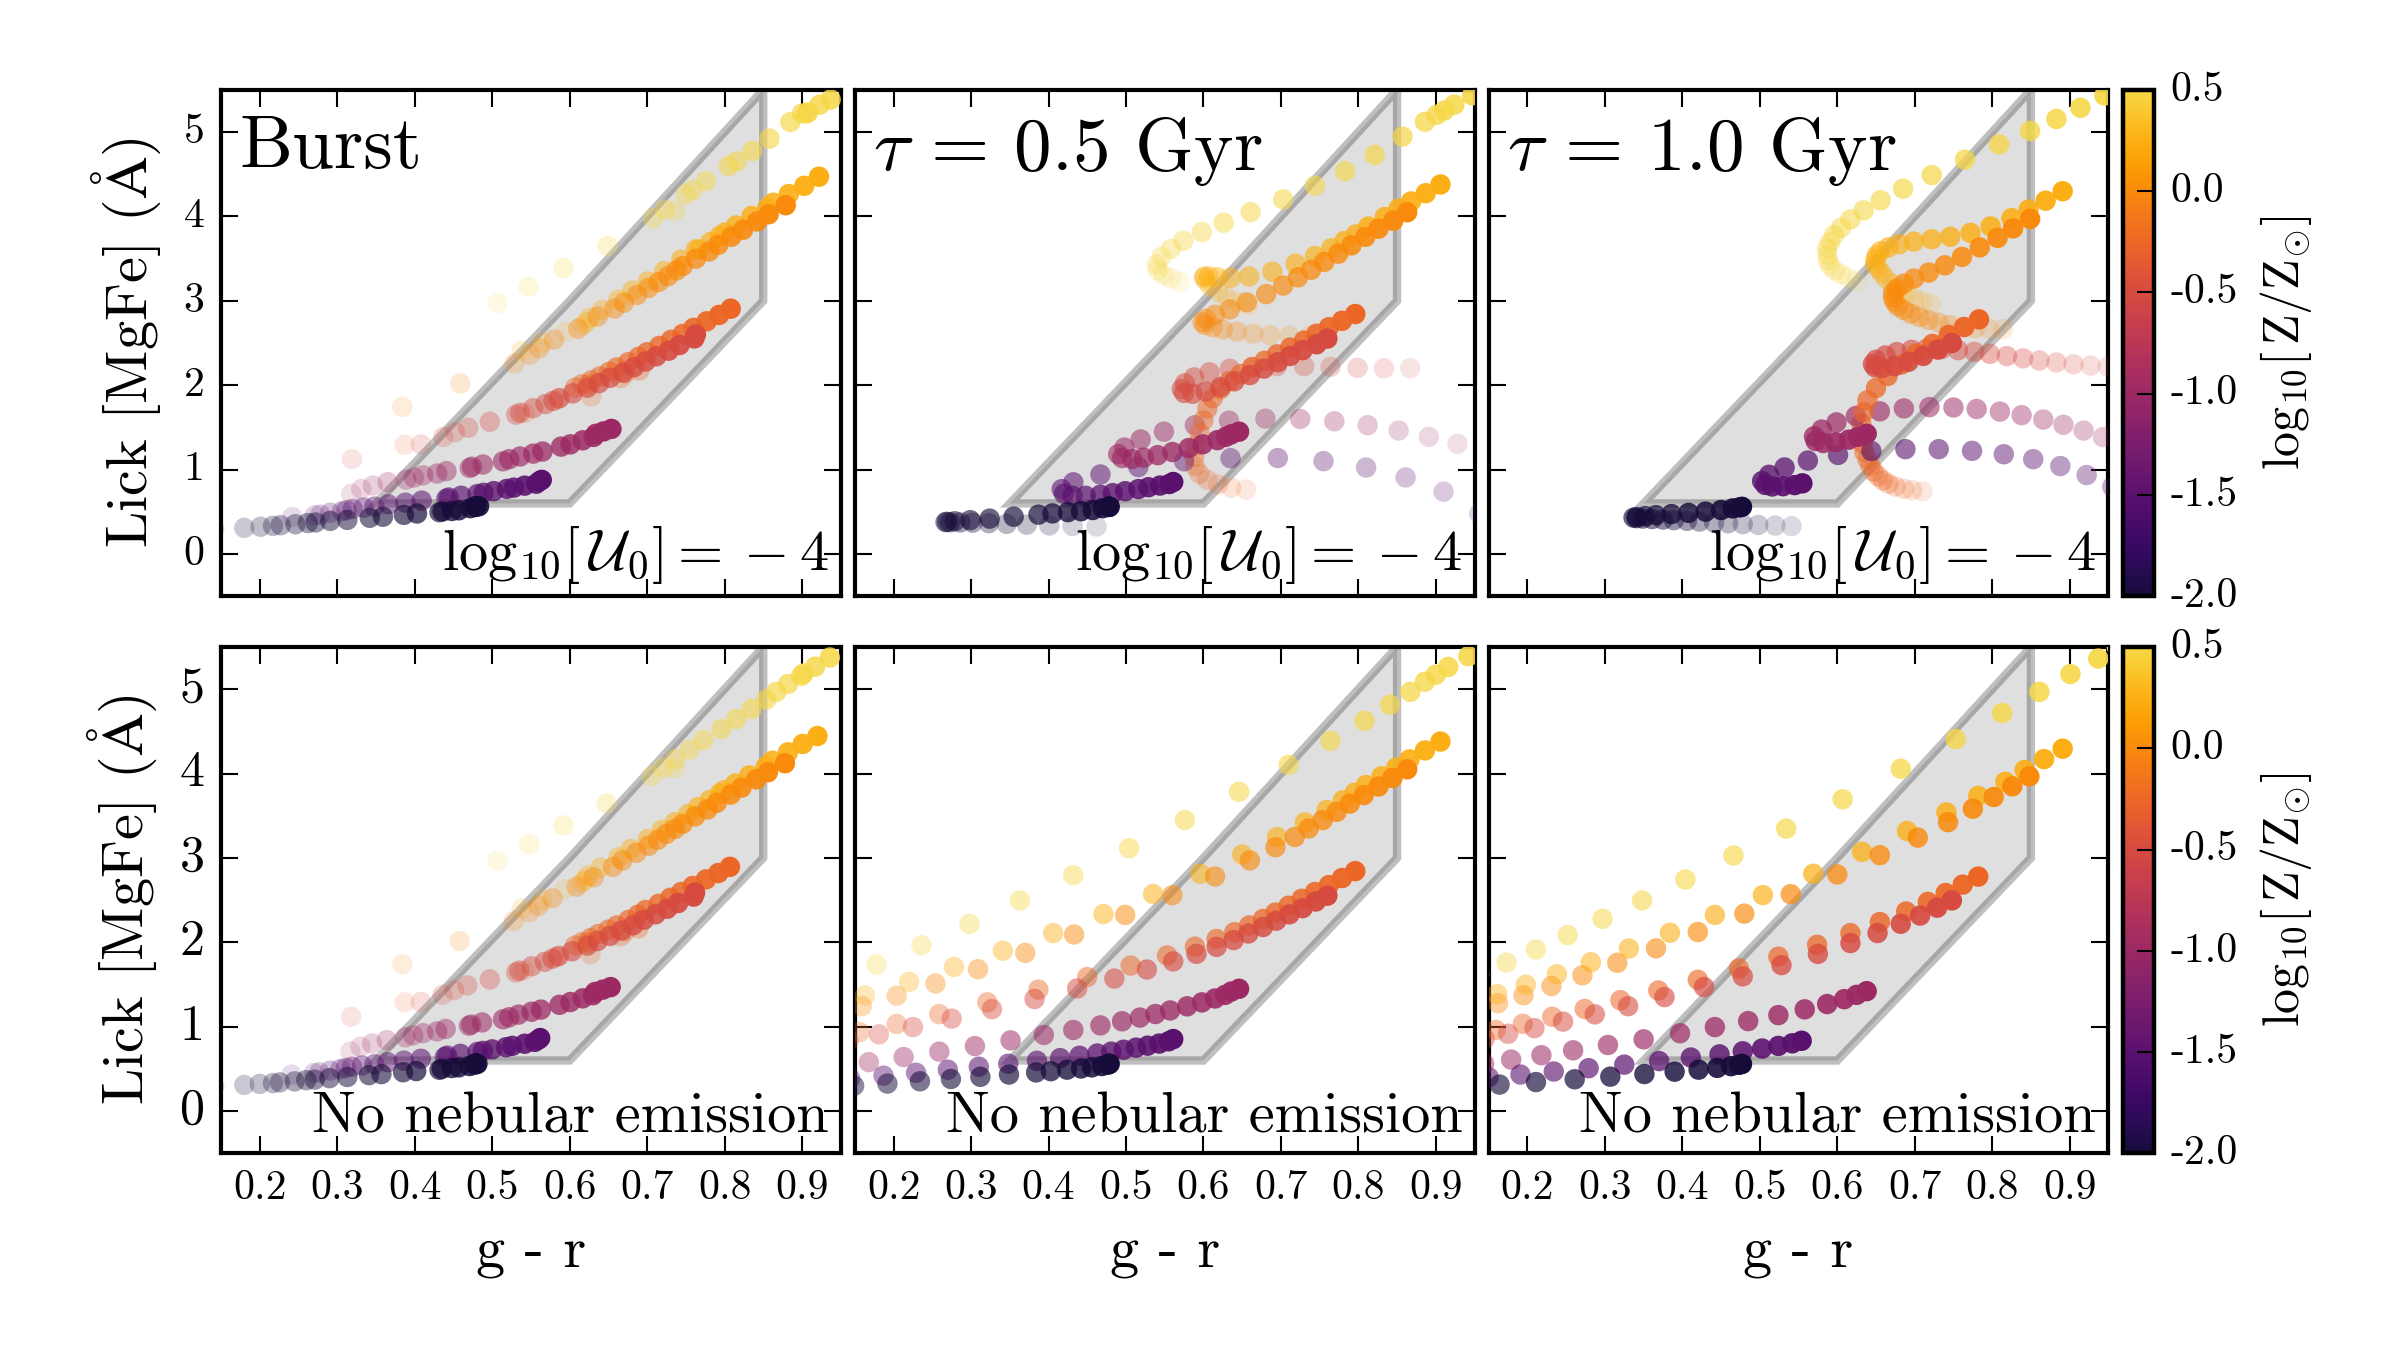
\includegraphics[width=\linewidth]{figs/f10.png}
    \caption{Optical $g-r$ color and the [MgFe] Lick index for our ETG models with stellar and nebular emission (\emph{top row}) and stellar only emission (\emph{bottom row}). Each column shows a different delayed$-\tau$ model SFH: $\tau=0.0$\Gyr (instantaneous burst, \emph{left}), $\tau=0.1$\Gyr (\emph{middle}), and $\tau=0.5$\Gyr (\emph{right}), and $\tau=1$\Gyr (\emph{bottom row}). Models with ages between 1 and 13\Gyr are plotted, color-coded by metallicity. Age is indicated by the transparency of the points, with the 13\Gyr model points fully opaque. The grey shaded region shows the location of observed objects from \citet{Schombert+2016}, which includes globular clusters and elliptical galaxies. For models with extended SF ($\tau=1$\Gyr), the inclusion of nebular emission alters the $g-r$ color at young ages. After $\sim5$\Gyr the models with nebular emission are consistent with the observed population of ETGs.
    }
    \label{fig:LickMgFe}
  \end{center}
\end{figure*}
%-------------------------------------------------------

%-------------------------------------------------------
% optical colors
%-------------------------------------------------------
\begin{figure*}
  \begin{center}
    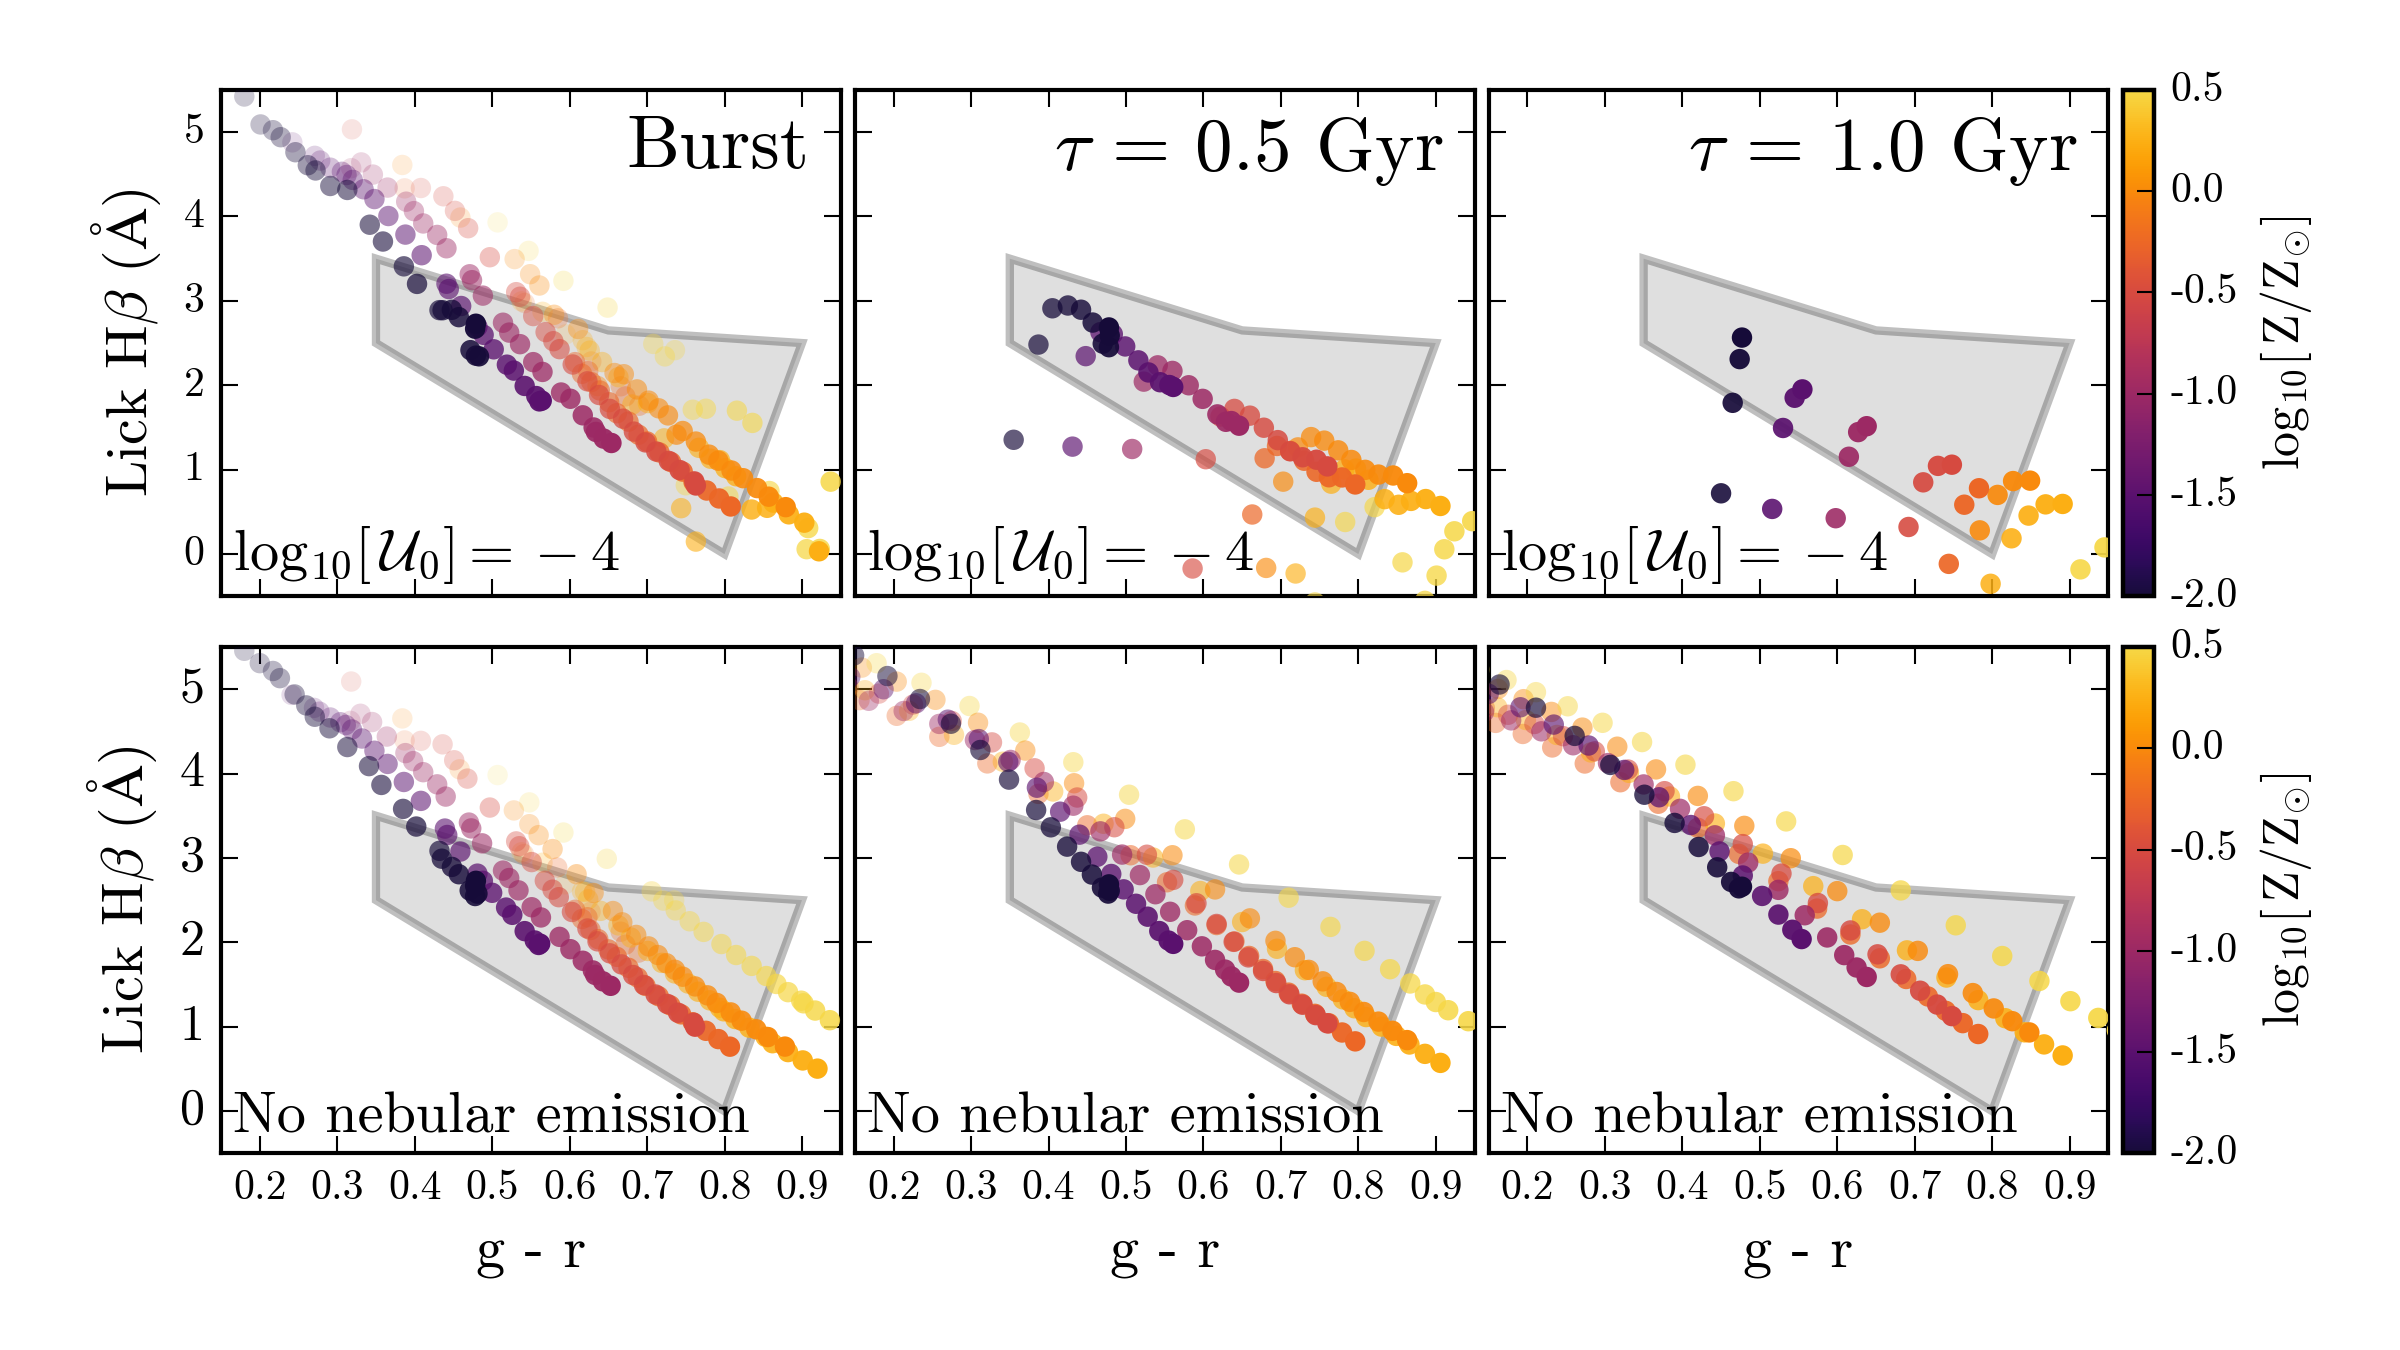
\includegraphics[width=\linewidth]{figs/f11.png}
    \caption{Optical $g-r$ color and the \hb Lick index for our ETG models with stellar and nebular emission (\emph{top row}) and stellar only emission (\emph{bottom row}). Each column shows a different delayed$-\tau$ model SFH: $\tau=0.0$\Gyr (instantaneous burst, \emph{left}), $\tau=0.1$\Gyr (\emph{middle}), and $\tau=0.5$\Gyr (\emph{right}). Models with ages between 1 and 13\Gyr are plotted, color-coded by metallicity. Age is indicated by the transparency of the points, with the 13\Gyr model points fully opaque. The grey shaded region shows the location of observed objects from \citet{Schombert+2016}, which includes globular clusters and elliptical galaxies. Nebular emission has an significant impact on the \hb index, since the emission fills in the \hb absorption feature, lowering the index.
    }
    \label{fig:LickHb}
  \end{center}
\end{figure*}
%-------------------------------------------------------

\subsection{LIER models with self-consistent colors and emission line properties} \label{sec:stars:EW:sfh}

We compare the \ha equivalent widths as a function of time for the delayed-$\tau$ models in Fig.~\ref{fig:EWtau}. Each panel shows a different model SFH at a range of metallicities, assuming \logUeq{-4}. For the models at \logUeq{-4}, the equivalent widths range from 0.1 to 5\ang at ages 1\Gyr and older. Larger values of $\tau$ produce a larger range in \ha EWs, especially at younger ages.

As shown in Figs.~\ref{fig:optCols}-\ref{fig:LickHb}, the main effect of SFH is to change the age at which a model looks like an ETG. Larger values of $\tau$ extend the duration of SF in a model, and these models do not look like ETGs until much later than the instantaneous bursts. The instantaneous bursts have ``ETG-like'' colors after $\sim3$\Gyr, while the models with $\tau$=1\Gyr only have ``ETG-like'' colors after 8\Gyr. The large EWs found in the $\tau$=1\Gyr models of Fig.~\ref{fig:EWtau} (right panel) are associated with contamination from residual star formation.

We have demonstrated that there are a broad range of model ages, SFHs, and metallicities that are able to reproduce the optical colors and absorption indices of ETGs. We now assess the emission line properties of the subset of models with optical spectra that ``look'' like ETGs. For the full grid of models that include nebular emission, we determine if the resultant broad-band colors are consistent with the observed range of ETGs, as determined using the region shown in Fig.~\ref{fig:optCols}, defined by \citet{Holden+2012} and updated by \citet{McIntosh+2014}.

We show \ha EWs for the delayed-$\tau$ models with ``ETG-like'' optical properties in Fig.~\ref{fig:linearEW}.
The top panel shows the time evolution of \ha equivalent widths at several metallicities, masking out all models that do not have ETG-like colors. Only models with metallicities of \logZeq{-1} and higher have colors consistent with the general ETG population. These models have \ha equivalent widths that vary from 0.1 to 3\ang with age, metallicity, and SFH.

The lower left panel of Fig.~\ref{fig:linearEW} shows the variation of \ha equivalent widths with metallicity, for models at $\log t = 10$ (10\Gyr) and a range of ionization parameters. We highlight those models with ETG-like colors with circular markers. For $\tau$=0.1 and 0.5\Gyr, the range of \ha equivalent widths is quite small, varying from 0.5 to 1\ang. For stellar populations at all metallicities, the post-AGB population has very similar temperatures, producing ionizing spectra with similar hardness. We thus expect that the models have similar ionization states, producing similar emission line ratios, as demonstrated in Figs.~\ref{fig:BPT1}-\ref{fig:BPT3}. 

Metallicity does change the emission properties of the models in two subtle ways. First, metallicity changes the underlying stellar continuum, and thus the \ha equivalent width. As shown in Fig.~\ref{fig:ionSpec}, lower metallicity models are brighter and hotter in the optical, and will have a larger contribution from the continuum. For a fixed number of ionizing photons, a larger continuum contribution produces smaller equivalent widths. Fig.~\ref{fig:EWtau} shows some evidence of larger EWs in higher metallicity models. Second, the lower metallicity models have more ionizing photons per unit stellar mass, and will thus produce more \ha emission. Fig.~\ref{fig:EWtau} shows some evidence of larger EWs at the lowest metallicities, but we note that these models do not produce optical colors that are consistent with the general ETG population.

Fig.~\ref{fig:linearEW} also shows the variation of the \ha equivalent width as a function of ionization parameter. The behavior is as expected here, where models with higher ionization parameters produce larger \ha equivalent widths. However, the range of EW is quite modest in spite of the large variation in \U, with the \ha EWs varying by only 15\% as the ionization parameter changes by 2 orders of magnitude. This suggests that although \U is a significant uncertainty in our physical model, the predictions of \ha EWs are relatively insensitive to the exact value of \U. In the model with $\tau$=1\Gyr, variation in ionization paramter produces a larger range in \ha EWs, due to the residual star formation.

%-------------------------------------------------------
% Tau models: Ha EW time evolution
%-------------------------------------------------------
\begin{figure*}
  \begin{center}
    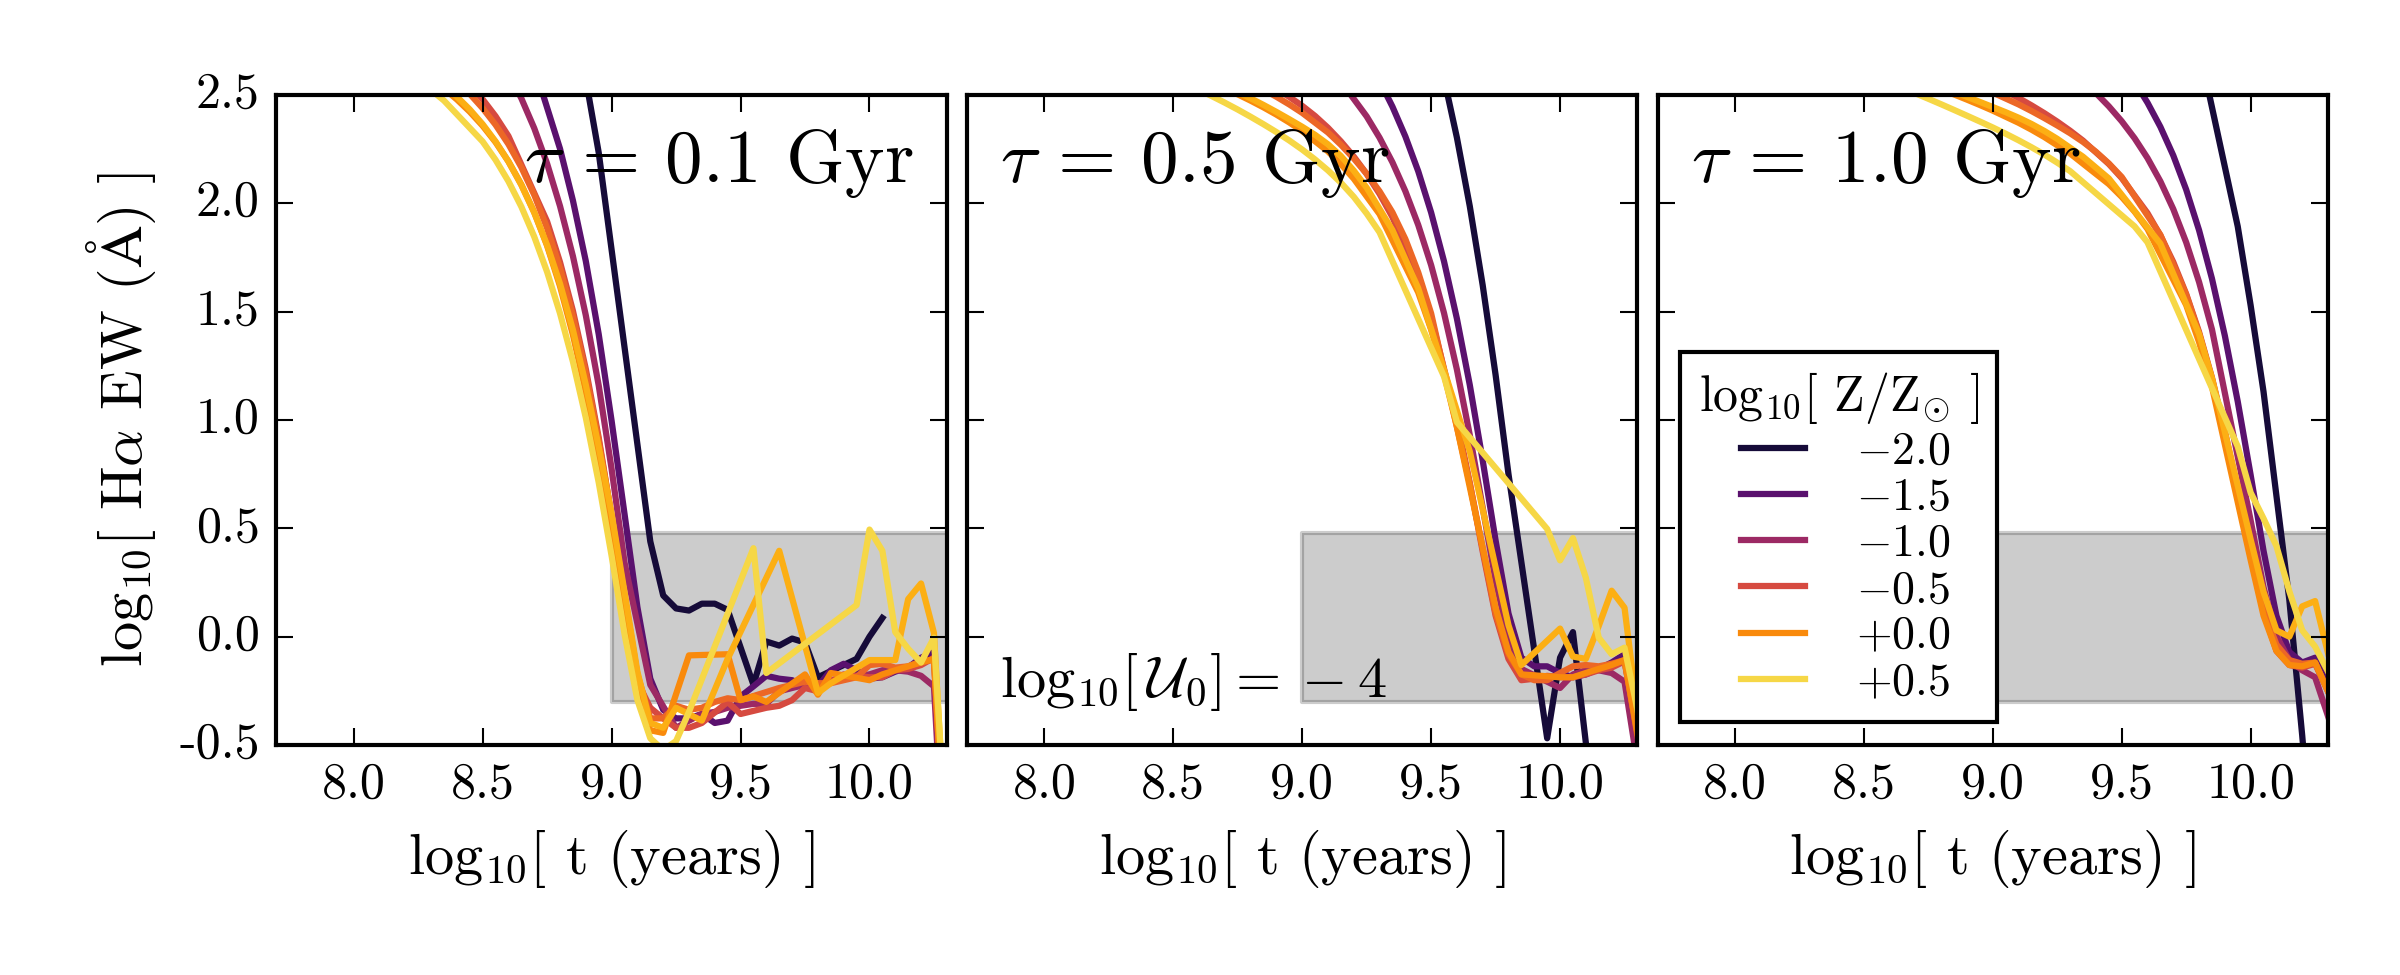
\includegraphics[width=\linewidth]{figs/f12.png}
    \caption{The time evolution of \ha equivalent widths for the delayed-$\tau$ models for $\tau=0.1$\Gyr (\emph{left}),  $\tau=0.5$\Gyr (\emph{middle}), and $\tau=1.0$\Gyr (\emph{right}). Metallicity varies from \logZeq{-2} in dark purple to \logZeq{0.5} in yellow. The grey shaded region highlights \ha EWs observed in typical LIER-like galaxies, of order $0.1-3\,$\ang.}
    \label{fig:EWtau}
  \end{center}
\end{figure*}
%-------------------------------------------------------

To briefly summarize, our models that include nebular emission are able to reproduce the optical properties of the general ETG population over a range of ages, SFHs, and metallicities. We find that instantaneous bursts and delayed-$\tau$ models with $\tau$=0.1, 0.5\Gyr, ages older than 3\Gyr, and metallicities between \logZeq{-1} and \logZeq{0.25} produce the most consistent combination of optical colors and Lick indices when compared with ETGs. This same subset of models produces \ha equivalent widths of order 0.1-3\ang, consistent with LIER-like galaxies. We find some evidence for higher \ha equivalent widths in higher metallicity models and models with higher ionization parameters, but in general the \ha EW is far more sensitive to age and SFH than either metallicity or \U.

%-------------------------------------------------------
% Tau models: LINEAR Ha EW time evolution
%-------------------------------------------------------
\begin{figure*}
  \begin{center}
    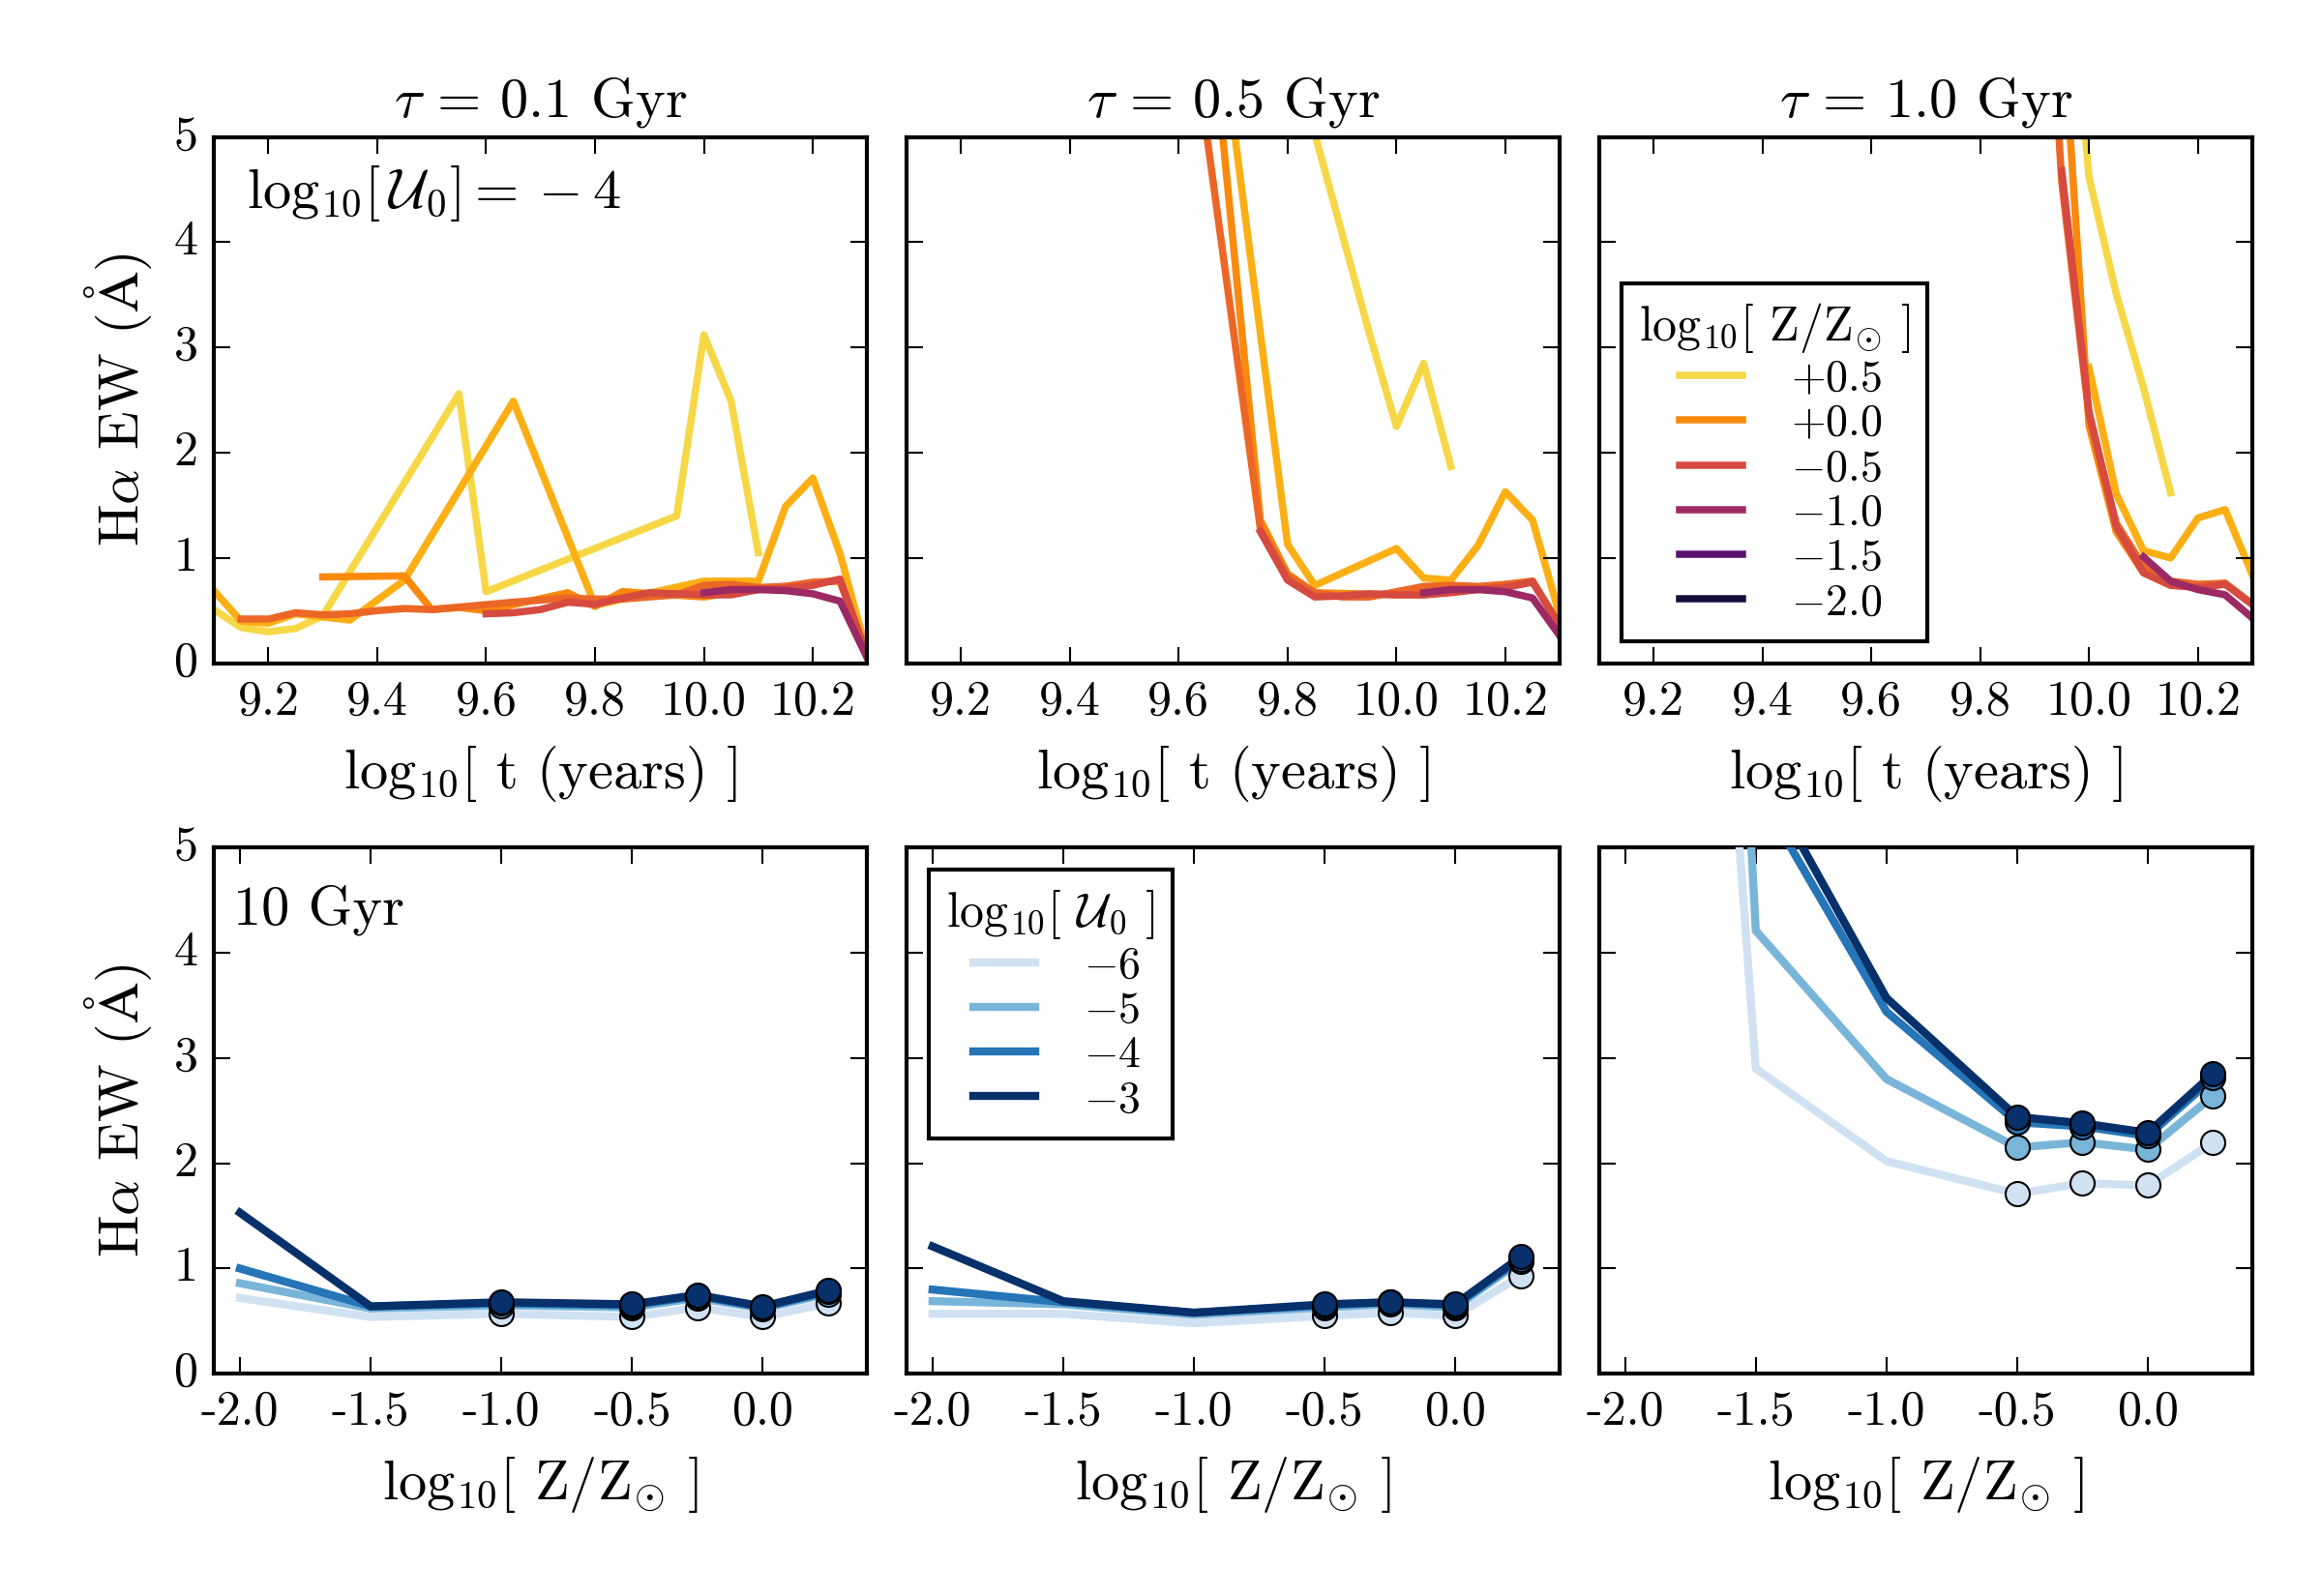
\includegraphics[width=\linewidth]{figs/f13.png}
    \caption{\emph{Top:} The time evolution of \ha equivalent widths for the subset of models with optical colors consistent with the general ETG population. The columns show $\tau=0.1$\Gyr (\emph{left}),  $\tau=0.5$\Gyr (\emph{middle}), and $\tau=1.0$\Gyr (\emph{right}). Metallicity varies from \logZeq{-2} in dark purple to \logZeq{0.5} in yellow; only the models with metallicities above \logZeq{-1.0} have ETG-like colors and LIER-like EWs. \emph{Bottom:} \ha equivalent widths as a function of metallicity for for $\tau=0.1$\Gyr (\emph{left}),  $\tau=0.5$\Gyr (\emph{middle}), and $\tau=1.0$\Gyr (\emph{right}). Ionization parameter is varied from \logUeq{-6} in light blue to \logUeq{-3} in dark blue. The subset of models with consistent ETG colors are highlighted with the circle markers.}
    \label{fig:linearEW}
  \end{center}
\end{figure*}
%-------------------------------------------------------

%%%%%%%%%%%%%%%%%%%%%%%%%%%%%%%%%%%%%%%%%%%%%%%%%%%%%%%%%%%%%%%%%%%%%%%%%%%%%%%%
%===============================================================================
\section{Conclusions}\label{sec:conclusions}
%===============================================================================

In this work, we present the first prediction of LIER-like emission from post-AGB stars that is based on fully self-consistent stellar models and photoionization modelling. We use these models to characterize the physical origin of LIER-like emission and post-AGB stars as an ionizing source. We have shown that evolved stellar populations where post-AGB stars provide the ionizing radiation source successfully reproduce LIER-like emission line ratios and \ha equivalent widths. These same models simultaneously reproduce the optical colors and absorption features observed in the general ETG population. We summarize our conclusions below.

\begin{itemize}
    \item For instantaneous bursts, post-AGB stars make up more than 95\% of the ionizing flux after ${\sim}100$\Myr, while horizontal branch stars never contribute more than 10\% of the total ionizing flux, assuming the default \FSPS parameters.
    \item Post-AGB star models produce emission line ratios consistent with LIER-like emission in the standard BPT diagram, the \sii/\ha diagram, and the \oi/\ha diagram.
    \item Post-AGB star models produce \ha equivalent widths between 0.1 and 10\ang, depending on the age, SFH, metallicity, and ionization parameter of the model.
    \item Post-AGB stars have very similar ionizing spectra at all metallicities. The similar hardness in the ionizing spectrum produces gas with similar ionization states, thus, emission line ratios from post-AGB stars do not vary much with stellar metallicity. The metallicity of the stellar population does, however, change the measured equivalent widths, since the underlying stellar continuum varies with metallicity as does the absolute number of ionizing photons produced per solar mass.
    \item Our models that include nebular emission are able to reproduce the optical properties of the general ETG population over a range of ages, SFHs, and metallicities. We find that instantaneous bursts and delayed-$\tau$ models with $\tau \lesssim 0.5$\Gyr, ages above 3\Gyr, and metallicities between \logZeq{-1} and \logZeq{0.25} produce the most consistent combination of optical colors and Lick indices when compared with ETGs. This same subset of models produces \ha equivalent widths of order 0.1-3\ang for \logUeq{-4}, consistent with LIER-like galaxies. Models with higher ionization parameters produce larger \ha equivalent widths, and we find some evidence for higher \ha equivalent widths in higher metallicity models.
\end{itemize}

We have demonstrated that the self-consistent stellar models for post-AGB stars have optical properties consistent with ETG galaxies. The optical properties of ETGs are fairly well understood, but the UV is much more uncertain, as galaxies with similar optical colors can have very different UV colors. In future work we will determine if the models presented here are also able to correctly predict the UV properties of ETGs, including the UV-excess observed in some ETGs.

%%%%%%%%%%%%%%%%%%%%%%%%%%%%%%%%%%%%%%%%%%%%%%%%%%%%%%%%%%%%%%%%%%%%%%%%%%%%%%%%
%-------------------------------------------------------
\bibliographystyle{aasjournal}
\bibliography{main}
%-------------------------------------------------------
\end{document}
